%! TEX program = xelatex
% 
% Template Proposal Tugas Akhir
% Program Studi Sistem dan Teknologi Informasi
% Sekolah Teknik Elektro dan Informatika
% Institut Teknologi Bandung
% 
% Dibuat oleh: IGB Baskara Nugraha 
% Email: baskara@itb.ac.id 
% 
% Last updated: 20 Oktober 2025
%
% Petunjuk penggunaan:
% 1. Ada 2 file utama, yaitu ProposalTA.tex (file ini) dan daftar-pustaka.bib (file daftar pustaka).
% 2. Sunting ProposalTA.tex sesuai dengan kebutuhan Anda.
% 3. Sunting atau generate isi daftar-pustaka.bib dengan referensi yang Anda gunakan, sesuai dengan format BibLaTeX.
% 4. Simpan kedua file tersebut dalam satu folder yang sama.
% 5. Kompilasi file ProposalTA.tex menggunakan XeLaTeX dan Biber (lihat urutan cara kompilasi di bawah).
% 6. Hasil kompilasi adalah file ProposalTA.pdf yang siap dicetak.
% 
% Urutan cara kompilasi (melalui command line):
% 1. xelatex ProposalTA.tex
% 2. biber ProposalTA      
% 3. xelatex  ProposalTA.tex
% 4. xelatex  ProposalTA.tex
%
% Catatan:
% - Pastikan Anda telah menginstal paket-paket LaTeX yang diperlukan, termasuk
%   biblatex-chicago dan fontspec.
% - Gunakan editor LaTeX yang mendukung XeLaTeX, seperti TeXstudio, Overleaf, atau lainnya.
% - Jika meenggunakan Visual Studio Code sebagai editor, pastikan mengatur "latex-workshop.latex.tools" dan
%   "latex-workshop.latex.recipes" untuk mendukung XeLaTeX dan Biber dengan cara menambahkan konfigurasi berikut:
%   "latex-workshop.latex.tools": [ 
%       {
%           "name": "xelatex",
%           "command": "xelatex",
%           "args": [
%               "-synctex=1",
%               "-interaction=nonstopmode",
%               "-file-line-error",
%               "%DOC%"
%           ]
%       },
%       {
%           "name": "biber",
%           "command": "biber",
%           "args": [
%               "%DOCFILE%"
%           ]
%       }
%   ],
%   "latex-workshop.latex.recipes": [
%       {
%           "name": "xelatex -> biber -> xelatex*2",
%           "tools": [
%               "xelatex",
%               "biber",
%               "xelatex",
%               "xelatex"
%           ]
%       }
%   ]
% - Untuk referensi lebih lanjut tentang penggunaan BibLaTeX dengan gaya Chicago, silakan merujuk ke dokumentasi resmi BibLaTeX.
%   https://ctan.org/pkg/biblatex-chicago
% - Untuk referensi lebih lanjut tentang penggunaan XeLaTeX dan fontspec, silakan merujuk ke dokumentasi resmi fontspec.
%   https://ctan.org/pkg/fontspec
% - Selamat menyusun proposal tugas akhir Anda!
%
\documentclass[12pt,a4paper,oneside]{book}

% ==========================================
% BASIC PACKAGES
% ==========================================
\usepackage[utf8]{inputenc} % for UTF-8 encoding
\usepackage{fontspec} % for font selection
\setmainfont{Times New Roman} % set main font to Times New Roman
\usepackage[a4paper, left=4cm, right=3cm, top=3cm, bottom=3cm]{geometry} % set page margins
\usepackage[indonesian]{babel} % untuk bahasa Indonesia
\usepackage{csquotes} % for context-sensitive quotation facilities
\usepackage{setspace} % for line spacing
\onehalfspacing % spasi 1.5
\usepackage{graphicx} % for images
\usepackage{caption} % for customizing captions
\usepackage{subcaption} % for sub-figures
\usepackage{hyperref} % for hyperlinks
\usepackage{titlesec} % for customizing titles
\usepackage{tocloft} % for customizing table of contents
\usepackage{lipsum} % for dummy text (lorem ipsum text)
\usepackage{floatrow} % for customizing float (figure and table) positions
\usepackage{listings} % for code listing
\usepackage{amsmath} % for math
\usepackage{amssymb} % for math symbols
\usepackage[shortlabels]{enumitem} % for customizing lists
\setlist[enumerate]{nosep, topsep=-10pt} % mengurangi spasi antar item dan atas bawah daftar
\setlist[itemize]{nosep, topsep=-10pt} % mengurangi spasi antar item dan atas bawah daftar
\usepackage[skip=12pt]{parskip}
\usepackage{longtable}
\usepackage{booktabs}
\usepackage[id-ID]{datetime2}


\setcounter{tocdepth}{4} % kedalaman daftar isi sampai subsubbab
\setcounter{secnumdepth}{4} % kedalaman penomoran sampai subsubbab


% ==========================================
% SITASI DAN DAFTAR PUSTAKA (MENGGUNAKAN CHICAGO MANUAL OF STYLE)
% ==========================================
\usepackage[
    backend=biber,
    authordate,
    language=english,
    autolang=other
]{biblatex-chicago}

\addbibresource{daftar-pustaka.bib}

% ==========================================
% Ubah istilah bahasa Inggris di daftar pustaka ke Bahasa Indonesia
% ==========================================
\DefineBibliographyStrings{english}{
  and          = {dan},
  andothers    = {dkk.},
  editor       = {penyunting},
  editors      = {penyunting},
  translator   = {penerjemah},
  byeditor     = {disunting oleh},
  bytranslator = {diterjemahkan oleh},
  in           = {dalam},
  edition      = {edisi},
  pages        = {hal.},
  page         = {hal.},
  volume       = {vol.},
  number       = {no.},
  urlseen      = {diakses pada},
  url          = {tautan},
}

% ==========================================
% Pastikan \cite() menampilkan (Penulis Tahun)
% ==========================================
\let\oldcite\cite
\renewcommand{\cite}{\parencite}

% ==========================================
% Atur pemisah nama penulis agar lebih natural dalam Bahasa Indonesia
% ==========================================
\renewcommand*{\finalandcomma}{} % hilangkan koma sebelum 'dan'


% ==========================================
% TAMPILAN
% ==========================================
\hypersetup{
    colorlinks=true,
    linkcolor=black,
    citecolor=black,
    urlcolor=black
}

% -- No Header dan No Footer ---
\pagestyle{plain}

% --- Ubah nama daftar listing ke "DAFTAR ALGORITMA" ---
% --- Harus diletakkan sebelum \begin{document} ---
\renewcommand{\lstlistlistingname}{\centering\normalsize DAFTAR KODE} 
\renewcommand{\lstlistingname}{Kode}
\lstset{basicstyle=\ttfamily\footnotesize,breaklines=true}
%\captionsetup[lstlisting]{justification=raggedright,singlelinecheck=false}


\renewcommand \cftchapdotsep{4.5}

% ==========================================
% AWAL DOKUMEN
% ==========================================
\begin{document}

% ==========================================
% HALAMAN JUDUL
% ==========================================
\begin{titlepage}
\begin{center}

    
    \vspace*{2cm}
    
    {\Large\bfseries SISTEM RANGKUMAN OTOMATIS BERBASIS AI UNTUK REDUKSI INFORMATION OVERLOAD DALAM KOMUNITAS FINANSIAL TELEGRAM BERJENJANG}\\
     \vspace{4cm}

    {\Large \textbf{Proposal Tugas Akhir}}\\


    \vspace{2cm}
    
    
    {\large Oleh}\\[0.3cm]
    \textbf{
    {\large Jonathan Wiguna}\\
    {\large 18222019}
    }\\

    \vspace{2cm}
    
    \begin{figure}[h]
    \centering
    \includegraphics[width=0.2\textwidth]{image/ganesha.jpg}
    \end{figure}
    
    
    % \vspace{1cm}
    \vfill

    \textbf{
    {\large PROGRAM STUDI SISTEM DAN TEKNOLOGI INFORMASI}\\
    {\large SEKOLAH TEKNIK ELEKTRO DAN INFORMATIKA}\\
    {\large INSTITUT TEKNOLOGI BANDUNG}\\
    {\large \DTMlangsetup{showdayofmonth=false,showmonthname=true,showyear=true}\today}
    }
\end{center}
\end{titlepage}



% ==========================================
% LEMBAR PENGESAHAN 
% ==========================================
\newpage
\thispagestyle{empty}
\pagenumbering{gobble}
\begin{center}
  \textbf{\large LEMBAR PENGESAHAN}\\[1cm]
  \vspace*{1.5cm}
    
  {\large\bfseries SISTEM RANGKUMAN OTOMATIS BERBASIS AI UNTUK REDUKSI INFORMATION OVERLOAD DALAM KOMUNITAS FINANSIAL TELEGRAM BERJENJANG}\\
     \vspace{2cm}

  {\Large \textbf{Proposal Tugas Akhir}}\\


  \vspace{1.5cm}
    
    
  {\large Oleh}\\[0.3cm]
    \textbf{
    {\large Jonathan Wiguna}\\
    {\large 18222019}
  }\\
    
  \vspace{0.5cm}
 
  {\large Program Studi Sistem dan Teknologi Informasi}\\
  {\large Sekolah Teknik Elektro dan Informatika}\\
  {\large Institut Teknologi Bandung}\\

  \vspace{1.5cm}

  Proposal Tugas Akhir ini telah disetujui dan disahkan\\ 
  di Bandung, pada tanggal \today\\[1cm]

% ==========================================
% Versi 1 pembimbing (default)
% ==========================================
	Pembimbing  \\[3cm]
	Dr. Ir. John Doe, M.T.   \\[0.2cm]
	NIP. 123456789 
% ==========================================

\end{center}

\vspace{1cm}
\noindent

% ==========================================
% Jika ada 2 pembimbing TA, uncomment dan edit 
% tabular di bawah ini. Kemudian, comment out atau hapus
% bagian versi 1 pembimbing di atas.
% ==========================================

%\begin{tabular}{p{1cm}p{7cm}p{7cm}}
%   & Pembimbing 1 & Pembimbing 2 \\[3cm]
%   & Dr. Ir. John Doe, M.T. & Dr. Mary Doe, M.Sc. \\[0.2cm]
%   &  NIP. 123456789 & NIP. 987654321
%\end{tabular}



% -- Change page number style to roman ---
\pagenumbering{roman} 


% ==========================================
% DAFTAR ISI, TABEL, GAMBAR
% ==========================================
% --- DAFTAR ISI ---
\makeatletter
\renewcommand{\tableofcontents}{%
  \clearpage
  \thispagestyle{plain}% no header
  \begin{center}
    {\large\bfseries\MakeUppercase{\contentsname}\par}
  \end{center}
  \vskip 1em
  \@starttoc{toc}%
}
\makeatother

\newpage
\renewcommand{\cfttoctitlefont}{\hfill\large\bfseries\MakeUppercase}
\renewcommand{\cftaftertoctitle}{\hfill}
\tableofcontents
%\addcontentsline{toc}{chapter}{DAFTAR ISI}

% --- DAFTAR GAMBAR ---
\newpage
\renewcommand{\cftloftitlefont}{\hfill\large\bfseries\MakeUppercase}
\renewcommand{\cftafterloftitle}{\hfill}
\listoffigures
\addcontentsline{toc}{chapter}{DAFTAR GAMBAR}

% --- DAFTAR TABEL ---
\newpage
\renewcommand{\cftlottitlefont}{\hfill\large\bfseries\MakeUppercase}
\renewcommand{\cftafterlottitle}{\hfill}
\listoftables
\addcontentsline{toc}{chapter}{DAFTAR TABEL}

% --- DAFTAR LISTING (ALGORITMA, PSEUDOCODE, SOURCE CODE) ---
\newpage

\lstlistoflistings
\addcontentsline{toc}{chapter}{\lstlistlistingname}

\mainmatter
% --- FORMAT TAMPILAN JUDUL BAB, SUBBAB, JUDUL GAMBAR DAN TABEL ---
% --- Judul Bab ---
\titleformat{\chapter}[display]
      {\centering\normalfont\large\bfseries} % Commands for the entire chapter title
      {\MakeUppercase \chaptertitlename\ \thechapter}{0pt}{\large} % Chapter number format
\renewcommand\thechapter{\Roman{chapter}}
% --- Judul Subbab dan Subsubbab ---
\titleformat{\section}
	{\normalfont\bfseries}
	{\thesection}{1em}{}
\titleformat{\subsection}
	{\normalfont\bfseries}
	{\thesubsection}{1em}{}
\titleformat{\subsubsection}
	{\normalfont\bfseries}
	{\thesubsubsection}{1em}{}


% --- Format judul gambar dan tabel ---
\captionsetup[figure]{labelsep=space}
\captionsetup[table]{labelsep=space}
\floatsetup[table]{capposition=top}
\captionsetup[lstlisting]{labelsep=space}
\floatsetup[lstlisting]{capposition=top}

% --- Atur indentasi paragraf ---
\setlength{\parindent}{0pt}
% -- Change page number style to arabic ---
\pagenumbering{arabic} 

% ==========================================
% BAB I PENDAHULUAN
% ==========================================
\chapter{PENDAHULUAN}
\label{chap:pendahuluan}

Bab I adalah pendahuluan yang menceritakan keseluruhan isi dari tugas akhir. Bab ini diawali dengan penjelasan mengenai topik dan latar belakang tugas akhir, dilanjuti dengan rumusan masalah, tujuan tugas akhir, serta batasan masalah yang dibahas di tugas akhir. Selain itu, Bab I akan menjelaskan tentang pendekatan dan metode yang digunakan di metodologi.

% --- Latar Belakang ---
\section{Latar Belakang}
Revolusi digital telah memicu ledakan produksi data; volume data global diproyeksikan akan mencapai 181 zettabyte pada tahun 2025, meningkat drastis dari hanya 2 zettabyte pada tahun 2010 \autocite{idc2025}. Pertumbuhan ini melahirkan tantangan \textit{information overload}, di mana volume informasi melampaui kapasitas kognitif individu untuk memprosesnya \autocite{eppler2004}. Menurut \textit{Cognitive Load Theory}, kapasitas memori kerja manusia yang terbatas membuat kualitas pengambilan keputusan dapat menurun hingga 50\% saat dihadapkan pada beban informasi berlebih \autocite{sweller1988,arnold2023}.

Masalah ini menjadi akut dalam komunitas online di media sosial, di mana laju pesan yang tinggi dapat menenggelamkan informasi krusial \autocite{nematzadeh2019}. Konsekuensinya adalah atensi selektif hingga kelumpuhan dalam pengambilan keputusan \autocite{edmunds2000}. Fenomena ini relevan di Indonesia, di mana platform seperti Telegram telah menjadi ekosistem dominan untuk komunitas finansial berskala besar. Didukung oleh fitur seperti kapasitas grup hingga 200.000 anggota, Telegram menjadi medium pilihan dengan lebih dari 27 juta pengguna di Indonesia untuk diskusi investasi \textit{real-time} \autocite{statista2024,perlo2025}.

Dominasi Telegram ini berjalan paralel dengan lonjakan jumlah investor ritel di Indonesia, yang mencapai lebih dari 6 juta investor pada September 2024, dengan pertumbuhan 744.000 investor baru di tahun tersebut \autocite{bei2024}. Mayoritas investor baru ini adalah generasi muda yang sangat bergantung pada komunitas media sosial untuk pengambilan keputusan investasi \autocite{ojk2022,jema2023}. Ketergantungan ini menciptakan masalah dimana akses informasi justru berujung pada \textit{information overload} yang parah, sehingga investor kesulitan memilah sinyal berkualitas dari kebisingan informasi. Tantangan ini terefleksi secara nyata dalam komunitas finansial Michael Yeoh, yang memiliki lebih dari 22.000 anggota dalam struktur berjenjang (\textit{multi-tiered}), di mana fragmentasi informasi antar grup semakin memperburuk masalah.

Penelitian akademis sebelumnya cenderung berfokus pada analisis sentimen dari forum publik seperti X (Twitter) dan Reddit untuk tujuan prediksi pergerakan harga saham (misalnya, \textcite{bollen2011}; \textcite{sianipar2023}; \textcite{liew2021}). Sementara itu, solusi praktis seperti bot Telegram yang ada saat ini bersifat generik, tidak mampu melakukan sintesis lintas-grup, dan tidak dioptimalkan untuk domain finansial Indonesia yang spesifik (misalnya, \textcite{stars2023}; \textcite{panda2023}). Kedua pendekatan tersebut tidak dirancang untuk menyelesaikan masalah operasional internal sebuah komunitas.

Kondisi \textit{information overload} parah dan fragmentasi informasi akibat struktur komunitas berjenjang ini menyoroti permasalahan signifikan yang perlu diteliti. Fenomena ini tidak hanya berisiko mengurangi efektivitas anggota dalam mengambil keputusan investasi, tetapi juga mengikis nilai dari komunitas itu sendiri.

% --- Rumusan Masalah ---
\section{Rumusan Masalah}
Berdasarkan latar belakang yang telah diuraikan pada subbab I.1, rumusan masalah yang akan dibahas pada tugas akhir ini adalah:

\begin{enumerate}
\item Bagaimana \textit{information overload} dan fragmentasi informasi dalam komunitas finansial berjenjang (\textit{multi-tiered}) secara spesifik menghambat kemampuan anggota untuk mengekstraksi wawasan investasi yang relevan?
\item Bagaimana sebuah sistem rangkuman otomatis berbasis AI dapat dikembangkan dan dievaluasi efektivitasnya untuk mereduksi \textit{information overload} dengan melakukan sintesis intelijen lintas-grup di komunitas tersebut?
\end{enumerate}

% --- Tujuan ---
\section{Tujuan}
Berdasarkan latar belakang dan rumusan masalah yang telah dijelaskan, tujuan dari tugas akhir ini adalah:

\begin{enumerate}
\item Menganalisis dampak \textit{information overload} dan fragmentasi informasi terhadap efektivitas anggota dalam memperoleh wawasan investasi di dalam studi kasus komunitas yang diteliti.
\item Merancang, membangun, dan mengevaluasi sebuah \textit{prototype} rangkuman otomatis yang mampu melakukan sintesis intelijen lintas-grup untuk membuktikan efektivitasnya dalam mengurangi \textit{information overload}.
\end{enumerate}

% --- Batasan Masalah ---
\section{Batasan Masalah}
Batasan masalah digunakan untuk menjaga pelebaran dari pokok masalah dan mengarahkan tugas akhir menjadi lebih spesifik. Batasan masalah dari tugas akhir ini adalah:

\begin{enumerate}
\item Konteks penelitian dan implementasi sistem terbatas secara eksklusif pada ekosistem komunitas investasi Michael Yeoh di Telegram, yang terdiri dari tiga grup utama: MY Cuap Cuap, MY Swing Plan, dan MY Advanced Group.
\item Arsitektur sistem menggunakan tumpukan teknologi (\textit{technology stack}) yang telah ditentukan, meliputi model NLP \textit{indonesian-roberta-base-emotion-classifier} dan \textit{bert-base-indonesian-NER}, serta pemanfaatan Groq API dengan model bahasa Llama 3.1 70B untuk proses generasi rangkuman.
\item Keluaran (\textit{output}) utama dari sistem adalah rangkuman terstruktur yang dihasilkan secara periodik setiap jam (\textit{hourly summary}). Penelitian ini tidak mencakup pengembangan sistem peringatan (\textit{alert}) \textit{real-time} atau fitur percakapan interaktif.
\item Sumber data untuk analisis terbatas pada pesan berbasis teks yang ada di dalam grup-grup Telegram yang ditentukan. Sistem tidak mengintegrasikan sumber data eksternal seperti API harga saham \textit{real-time} atau umpan berita finansial dari portal media.
\end{enumerate}

% --- Metodologi Pengerjaan TA ---
\section{Metodologi}
Pengerjaan tugas akhir ini menggunakan dua metodologi, yaitu metodologi untuk penelitian dan metodologi pengembangan.

\subsection{Metodologi Penelitian}
Metodologi penelitian yang digunakan adalah \textit{Design Science Research Methodology} (DSRM). Pendekatan DSRM dipilih karena relevansinya yang tinggi dengan penelitian di bidang sistem informasi yang bertujuan untuk merancang dan mengevaluasi artefak teknologi inovatif guna memecahkan masalah di dunia nyata. Proses DSRM terdiri dari enam tahapan yang akan diikuti dalam penelitian ini:

\begin{enumerate}
\item \textbf{Identifikasi Masalah \& Motivasi}: Tahap ini telah diuraikan dalam latar belakang, di mana masalah spesifik yang diidentifikasi adalah \textit{information overload} dan fragmentasi informasi dalam komunitas finansial Telegram yang besar dan berjenjang. Motivasi utamanya adalah kebutuhan untuk meningkatkan efisiensi akses informasi bagi anggota komunitas.

\item \textbf{Perumusan Tujuan Solusi}: Berdasarkan masalah yang ada, tujuan solusi didefinisikan secara kuantitatif dan kualitatif. Tujuan utamanya adalah menghasilkan sebuah artefak (sistem) yang terbukti mampu mereduksi beban informasi, yang akan diukur melalui akurasi identifikasi topik dan efisiensi akses informasi yang dirasakan pengguna.

\item \textbf{Desain \& Pengembangan}: Tahap ini merupakan aktivitas inti dalam menciptakan artefak penelitian. Pada tugas akhir ini, artefak yang dirancang dan dikembangkan adalah sebuah sistem purwarupa untuk rangkuman otomatis. Proses ini mencakup perancangan arsitektur, implementasi \textit{pipeline} pemrosesan data, dan integrasi model NLP.

\item \textbf{Demonstrasi}: Pada tahap ini, artefak yang telah dibangun akan didemonstrasikan untuk menyelesaikan masalah yang telah diidentifikasi. Sistem purwarupa akan dioperasikan menggunakan data percakapan nyata dari komunitas Michael Yeoh untuk menunjukkan kemampuannya dalam mengubah data mentah menjadi rangkuman yang terstruktur.

\item \textbf{Evaluasi}: Artefak akan dievaluasi secara sistematis untuk mengukur sejauh mana tujuan solusi tercapai. Evaluasi akan membandingkan kondisi sebelum dan sesudah penggunaan sistem, menggunakan metrik yang telah ditetapkan seperti akurasi, tingkat kompresi pesan, dan umpan balik kualitatif dari pengguna melalui survei.

\item \textbf{Komunikasi}: Tahap terakhir adalah mengkomunikasikan masalah, artefak yang dibangun, serta hasil evaluasinya kepada audiens akademis. Komunikasi ini diwujudkan melalui penulisan laporan tugas akhir ini serta presentasi dalam forum seminar dan sidang.
\end{enumerate}

\subsection{Metodologi Pengembangan}
Metodologi pengembangan yang akan digunakan akan dijelaskan lebih detail pada tahap selanjutnya setelah analisis kebutuhan sistem dilakukan.

% ==========================================
% BAB II STUDI LITERATUR
% ==========================================
\chapter{STUDI LITERATUR}
\label{chap:studi-literatur}

Bab ini menyajikan tinjauan komprehensif terhadap literatur yang relevan dengan pengembangan sistem rangkuman otomatis berbasis \textit{AI} untuk mereduksi \textit{information overload} dalam komunitas finansial Telegram. Studi literatur ini mencakup tujuh domain utama: (1) \textit{Information Overload} dan \textit{Cognitive Load Theory}, (2) \textit{Text Summarization} dengan \textit{Large Language Models}, (3) Analisis Sentimen untuk Media Sosial Finansial, (4) \textit{Named Entity Recognition} untuk Teks Finansial Indonesia, (5) \textit{Topic Modeling} dengan BERTopic, (6) Telegram sebagai Platform Komunitas, dan (7) Arsitektur Pemrosesan Data \textit{Real-Time}. Setiap domain memberikan landasan teoretis dan metodologis yang mendukung desain, implementasi, dan evaluasi sistem yang dikembangkan dalam penelitian ini.

% ==========================================
\section{\textit{Information Overload} dan \textit{Cognitive Load Theory}}
\label{sec:information-overload}

\textit{Information overload} merupakan fenomena di mana individu dihadapkan pada volume informasi yang melampaui kapasitas kognitif mereka untuk memproses secara efektif \autocite{eppler2004}. Dalam konteks komunitas online, khususnya platform media sosial seperti Telegram, masalah ini menjadi semakin akut karena tingginya laju produksi dan distribusi informasi. Bagian ini mengulas teori-teori fundamental yang menjelaskan bagaimana \textit{information overload} memengaruhi pengambilan keputusan, serta mengidentifikasi strategi mitigasi yang dapat diterapkan melalui sistem otomatis berbasis \textit{AI}.

\subsection{Konsep dan Dampak \textit{Information Overload}}

Penelitian seminal oleh \textcite{eppler2004} menyediakan landasan teoretis yang komprehensif tentang konsep \textit{information overload}. Berdasarkan tinjauan literatur dari berbagai disiplin ilmu termasuk \textit{Organization Science}, Akuntansi, Pemasaran, dan Sistem Informasi Manajemen, mereka mendefinisikan \textit{information overload} sebagai kondisi di mana kualitas pengambilan keputusan menurun ketika kuantitas informasi yang tersedia melampaui kapasitas pemrosesan individu. Studi tersebut mengidentifikasi hubungan inverted U-curve antara kuantitas informasi dan kualitas keputusan, yang menunjukkan bahwa setelah mencapai titik optimal, penambahan informasi justru menurunkan performa kognitif. Temuan ini sangat relevan dengan konteks komunitas Telegram finansial yang menghasilkan ratusan hingga ribuan pesan per hari, yang berpotensi menempatkan anggota komunitas pada sisi kanan kurva tersebut di mana \textit{overload} terjadi.

\begin{figure}[H]
  \centering
  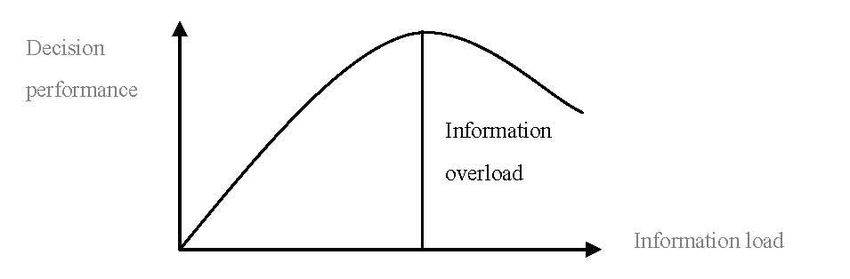
\includegraphics[width=0.7\textwidth]{image/information-overload-curve.png}
  \caption{Hubungan \textit{inverted U-curve} antara kuantitas informasi dan kualitas pengambilan keputusan, menunjukkan titik optimal dan zona \textit{overload} (diadaptasi dari \textcite{eppler2004})}
  \label{fig:info-overload}
\end{figure}

\textcite{shahrzadi2024} memperkuat pemahaman ini melalui \textit{scoping review} terbaru yang menganalisis penyebab, konsekuensi, dan strategi penanganan \textit{information overload}. Penelitian mereka mengidentifikasi tiga kategori penyebab utama: (1) faktor personal seperti keterbatasan kapasitas kognitif dan kurangnya keterampilan manajemen informasi, (2) karakteristik informasi seperti ambiguitas, kompleksitas, dan ketidakpastian, dan (3) parameter teknologi informasi termasuk intensitas notifikasi dan desain antarmuka. Dampak yang diidentifikasi mencakup penurunan produktivitas, kualitas keputusan yang buruk, stres, dan kelelahan kognitif. Yang paling signifikan bagi penelitian ini adalah identifikasi mereka terhadap strategi mitigasi berbasis teknologi, khususnya penggunaan \textit{filtering tools} dan sistem otomatis untuk mereduksi volume informasi, yang memberikan justifikasi langsung untuk pengembangan bot rangkuman otomatis.

\subsection{Landasan Teori: \textit{Cognitive Load Theory}}

\textit{Cognitive Load Theory} (CLT), yang dikembangkan oleh \textcite{sweller1988}, memberikan kerangka teoretis untuk memahami keterbatasan kapasitas memori kerja manusia dalam pemrosesan informasi. Teori ini mengidentifikasi tiga jenis beban kognitif: (1) \textit{intrinsic load}, yang inheren dengan kompleksitas materi yang dipelajari, (2) \textit{extraneous load}, yang dihasilkan oleh cara informasi disajikan, dan (3) \textit{germane load}, yang berkontribusi pada pembentukan skema dan otomatisasi. Dalam konteks komunitas online, anggota menghadapi \textit{intrinsic load} yang tinggi karena kompleksitas informasi finansial, sementara desain antarmuka platform media sosial sering kali meningkatkan \textit{extraneous load} melalui notifikasi, pesan yang tidak terstruktur, dan kurangnya organisasi informasi.

\begin{figure}[H]
  \centering
  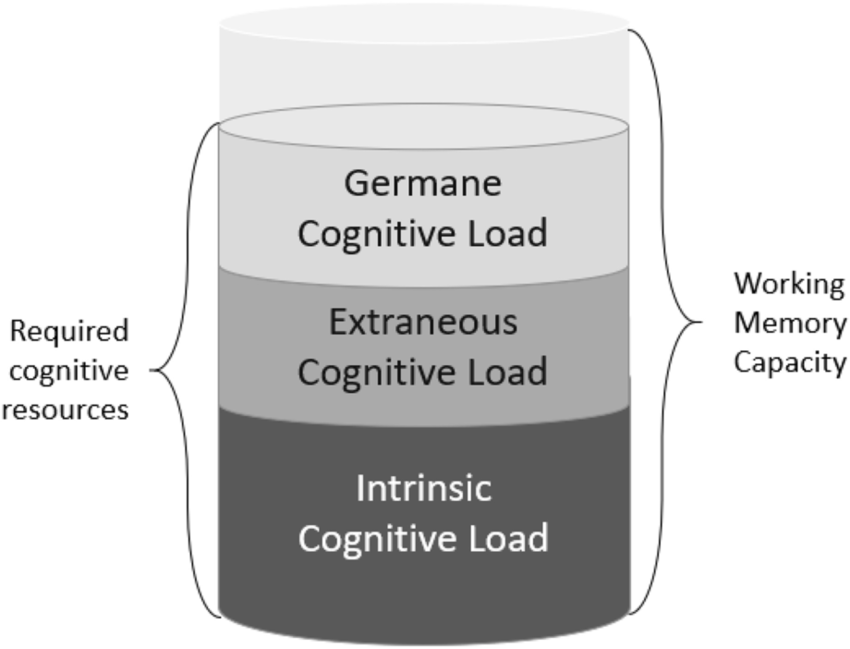
\includegraphics[width=0.75\textwidth]{image/cognitive-load-theory.png}
  \caption{Tiga jenis beban kognitif dalam \textit{Cognitive Load Theory}: \textit{intrinsic}, \textit{extraneous}, dan \textit{germane load} (diadaptasi dari \textcite{sweller1988})}
  \label{fig:cognitive-load}
\end{figure}

\textcite{skulmowski2022} mengembangkan pemahaman CLT dengan mengadaptasinya untuk lingkungan digital dan pembelajaran daring. Penelitian mereka mengusulkan perspektif baru tentang \textit{extraneous cognitive load} yang mempertimbangkan karakteristik unik media digital, seperti konten yang kaya secara perseptual, distraksi visual, dan desain antarmuka yang kompleks. Mereka berargumen bahwa media digital menciptakan bentuk \textit{extraneous load} yang berbeda dari media tradisional, terutama melalui elemen-elemen yang tidak relevan dengan tujuan pembelajaran atau pemrosesan informasi inti. Temuan ini sangat relevan untuk memahami bagaimana antarmuka Telegram yang penuh dengan pesan, emoji, dan media visual dapat meningkatkan beban kognitif ekstrinsik bagi anggota yang mencoba mengekstrak informasi investasi yang relevan.

Penelitian empiris oleh \textcite{sidnammauch2024} menerapkan CLT secara khusus pada konteks distraksi media sosial melalui studi dengan 1.026 partisipan. Mereka mengintegrasikan \textit{load theory of attention} dengan kerangka \textit{uses and gratifications} untuk menjelaskan bagaimana media sosial mobile menciptakan distraksi melalui sumber daya kognitif yang terbatas. Studi mereka mendemonstrasikan bahwa individu dengan kapasitas memori kerja yang lebih rendah lebih rentan terhadap distraksi media sosial, dan bahwa \textit{affordances} teknologi seperti notifikasi \textit{push} dan aksesibilitas konstan memperburuk masalah ini. Temuan ini memperkuat argumen bahwa komunitas Telegram finansial dengan lebih dari 22.000 anggota dan aliran pesan yang konstan menciptakan lingkungan yang sangat rentan terhadap \textit{cognitive overload} dan distraksi, yang pada akhirnya dapat menurunkan kualitas pengambilan keputusan investasi.

\subsection{Ekonomi Perhatian di Media Sosial}

\textcite{heitmayer2025} memberikan perspektif teoretis terbaru dengan mengusulkan bahwa perhatian (\textit{attention}) berfungsi sebagai mata uang simbolis universal di media sosial. Penelitian ini memperkenalkan model \textit{dual-stream} yang membedakan antara perhatian yang "mengalir" (\textit{flow attention}) dan perhatian yang "mengeras" (\textit{calcified attention}). \textit{Flow attention} mengacu pada alokasi perhatian yang dinamis dan sementara terhadap konten yang terus berubah, sementara \textit{calcified attention} merujuk pada investasi perhatian jangka panjang yang termanifestasi dalam bentuk \textit{followers}, \textit{likes}, atau keanggotaan komunitas. Dalam konteks komunitas finansial Telegram, kedua bentuk perhatian ini bersaing: anggota harus mengalokasikan \textit{flow attention} mereka untuk memproses aliran pesan yang konstan, sementara \textit{calcified attention} mereka termanifestasi dalam komitmen berkelanjutan terhadap komunitas dan kepercayaan terhadap sumber informasi tertentu seperti Michael Yeoh. Kelangkaan perhatian (\textit{attention scarcity}) yang diidentifikasi dalam penelitian ini menjadi masalah sentral yang harus diatasi oleh sistem rangkuman otomatis dengan memaksimalkan efisiensi alokasi perhatian anggota.

Analisis empiris oleh \textcite{nematzadeh2019} tentang \textit{information overload} dalam komunikasi grup menggunakan data dari platform Twitch menunjukkan bagaimana peningkatan volume pesan dalam grup dapat menyebabkan transisi dari percakapan yang koheren menjadi "kakofoni" di mana informasi bermakna tenggelam dalam kebisingan. Mereka mengidentifikasi bahwa ketika laju pesan melebihi ambang batas tertentu, kualitas percakapan menurun drastis, partisipasi menjadi tidak merata, dan informasi penting hilang. Fenomena ini sangat relevan dengan komunitas Telegram finansial yang diteliti, di mana pesan dapat muncul dengan laju ratusan per jam selama jam perdagangan aktif. Sistem rangkuman otomatis yang dirancang dalam penelitian ini bertujuan untuk mengatasi transisi menuju kakofoni ini dengan menyaring dan mensintesis informasi kunci secara periodik.


% ==========================================
\section{\textit{Text Summarization} dengan \textit{Large Language Models}}
\label{sec:text-summarization}

Peringkasan teks otomatis telah mengalami evolusi signifikan dengan munculnya model bahasa berbasis \textit{transformer} dan \textit{large language models} (LLMs). Bagian ini mengulas perkembangan metodologi peringkasan teks dari pendekatan berbasis ekstraksi hingga generasi abstraktif dengan LLMs, dengan fokus khusus pada tantangan peringkasan multi-dokumen dan percakapan yang relevan dengan konteks komunitas Telegram.

\subsection{Fondasi: Arsitektur \textit{Transformer} dan BERT}

Sebelum membahas aplikasi model bahasa dalam peringkasan teks, penting untuk memahami arsitektur fundamental yang mendasari perkembangan NLP modern: \textit{Transformer} dan \textit{Bidirectional Encoder Representations from Transformers} (BERT). Kedua inovasi ini telah merevolusi pemrosesan bahasa alami dan menjadi dasar bagi hampir semua model bahasa kontemporer yang digunakan dalam penelitian ini.

\textcite{vaswani2017} memperkenalkan arsitektur \textit{Transformer} yang menggantikan arsitektur rekuren tradisional (\textit{RNN}, \textit{LSTM}) dengan mekanisme \textit{self-attention} yang dapat memproses seluruh urutan input secara paralel. Inovasi kunci dari \textit{Transformer} adalah kemampuannya untuk menangkap dependensi jarak jauh dalam teks tanpa keterbatasan memori yang dialami oleh arsitektur rekuren. Mekanisme \textit{multi-head attention} memungkinkan model untuk menghadiri berbagai aspek representasional input secara simultan, sementara \textit{positional encoding} mempertahankan informasi tentang urutan kata. Arsitektur \textit{encoder-decoder} yang diusulkan terdiri dari tumpukan lapisan \textit{transformer} yang masing-masing mengandung sub-lapisan \textit{multi-head self-attention} dan \textit{feed-forward neural network}. Penelitian seminal ini mencapai hasil \textit{state-of-the-art} pada tugas terjemahan mesin dan menetapkan \textit{Transformer} sebagai arsitektur dominan untuk NLP.

\begin{figure}[H]
  \centering
  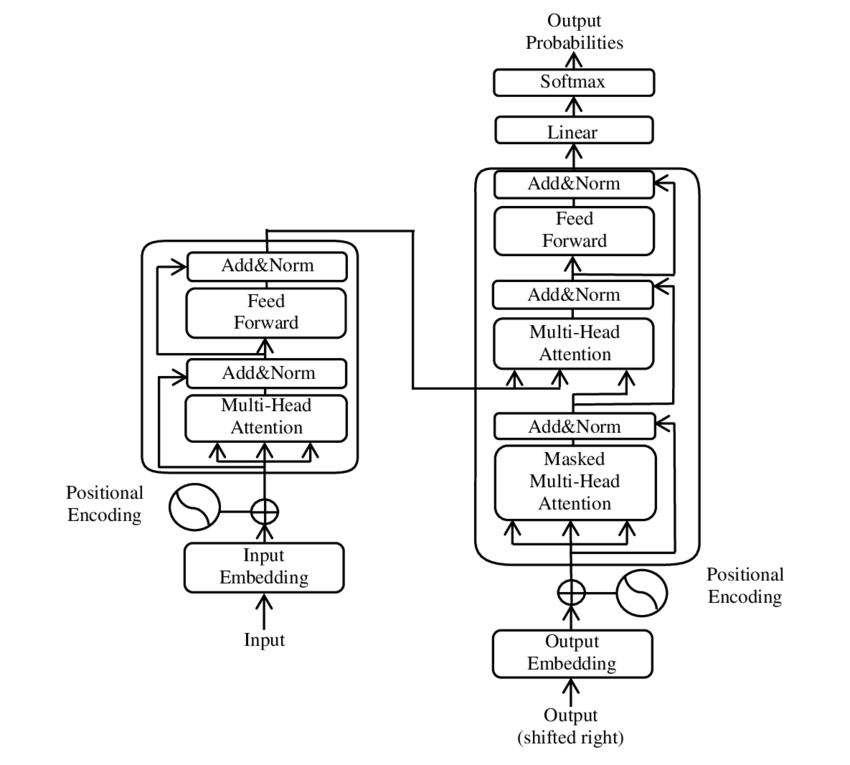
\includegraphics[width=0.65\textwidth]{image/transformer-architecture.png}
  \caption{Arsitektur Transformer dengan mekanisme \textit{multi-head attention} dan struktur \textit{encoder-decoder} (diadaptasi dari \textcite{vaswani2017})}
  \label{fig:transformer-arch}
\end{figure}

\textcite{devlin2019} mengembangkan konsep \textit{Transformer} lebih lanjut dengan memperkenalkan BERT (\textit{Bidirectional Encoder Representations from Transformers}), model bahasa yang dilatih secara \textit{bidirectional} menggunakan arsitektur \textit{Transformer encoder}. Berbeda dengan model bahasa unidirectional sebelumnya yang hanya memproses teks dari kiri ke kanan atau kanan ke kiri, BERT dilatih menggunakan dua tugas pra-latih: \textit{Masked Language Modeling} (MLM), di mana sebagian token input di-\textit{mask} dan model harus memprediksinya berdasarkan konteks bidirectional, dan \textit{Next Sentence Prediction} (NSP), di mana model memprediksi apakah dua kalimat berurutan dalam teks original. Pendekatan \textit{pre-training} dan \textit{fine-tuning} yang diusulkan memungkinkan BERT untuk mencapai performa \textit{state-of-the-art} pada sebelas tugas NLP yang beragam, termasuk klasifikasi teks, \textit{question answering}, dan \textit{natural language inference}. Representasi kontekstual bidirectional yang dihasilkan BERT menangkap nuansa semantik yang tidak dapat ditangkap oleh model unidirectional atau representasi statis seperti Word2Vec.

Gambar \ref{fig:bert-architecture} mengilustrasikan arsitektur BERT dan perbedaannya dengan model bahasa unidirectional. Arsitektur ini menjadi fondasi bagi berbagai varian yang digunakan dalam penelitian ini, termasuk IndoBERT untuk bahasa Indonesia, RoBERTa untuk klasifikasi emosi, dan model NER berbasis BERT untuk ekstraksi entitas finansial.

\begin{figure}[H]
  \centering
  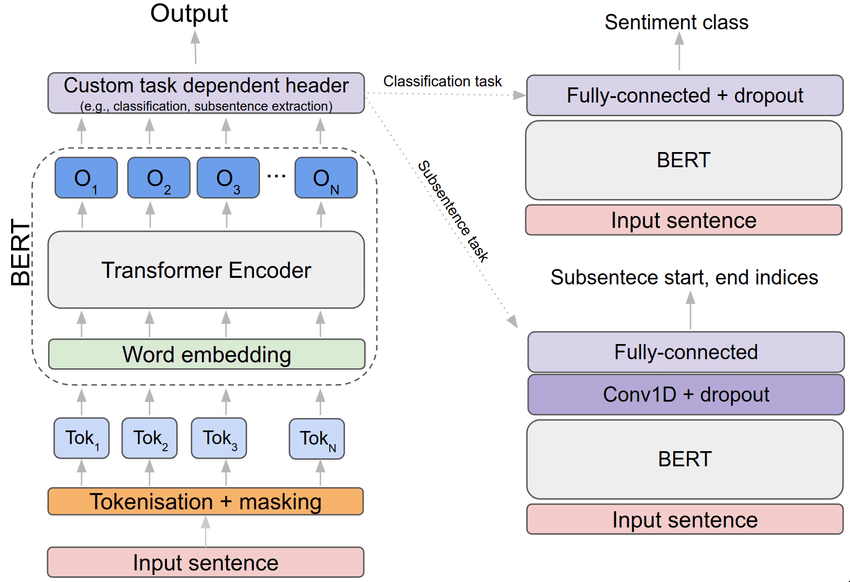
\includegraphics[width=0.85\textwidth]{image/bert-architecture-diagram.png}
  \caption{Arsitektur BERT menunjukkan mekanisme \textit{bidirectional self-attention} dan proses \textit{pre-training} dengan \textit{Masked Language Modeling} (diadaptasi dari \textcite{devlin2019})}
  \label{fig:bert-architecture}
\end{figure}

Kontribusi BERT terhadap NLP tidak hanya terletak pada performa superiornya pada berbagai \textit{benchmark}, tetapi juga pada paradigma \textit{transfer learning} yang efektif: model bahasa umum yang besar dilatih pada korpus teks masif, kemudian di-\textit{fine-tune} untuk tugas spesifik dengan data berlabel yang relatif terbatas. Paradigma ini sangat relevan dengan konteks penelitian ini, di mana model IndoBERT yang telah dilatih pada korpus bahasa Indonesia umum di-\textit{fine-tune} untuk tugas-tugas spesifik domain finansial seperti analisis sentimen dan ekstraksi entitas.

\subsection{Peringkasan Berbasis \textit{Transformer}}

\textcite{liu2019bertsum} memperkenalkan pendekatan \textit{BERTSum} yang memanfaatkan representasi BERT untuk peringkasan ekstraktif dan abstraktif. Penelitian mereka mendemonstrasikan bahwa model \textit{encoder} tingkat dokumen yang dibangun di atas BERT dengan lapisan \textit{Transformer} antar-kalimat dapat menghasilkan rangkuman berkualitas tinggi. Pendekatan dua tahap \textit{fine-tuning} yang mereka usulkan, di mana model pertama-tama di-\textit{fine-tune} untuk tugas ekstraksi kalimat sebelum dilatih untuk generasi abstraktif, menetapkan metodologi dasar yang diadopsi oleh banyak penelitian berikutnya. Kontribusi kunci dari penelitian ini adalah demonstrasi bahwa model bahasa pra-latih dapat secara efektif menangkap struktur dokumen dan hubungan semantik antar-kalimat, yang esensial untuk menghasilkan rangkuman yang koheren dan informatif.

Pemahaman tentang \textit{trade-off} antara peringkasan ekstraktif dan abstraktif diperluas oleh penelitian \textcite{pilault2020}, yang membandingkan kedua pendekatan menggunakan model \textit{transformer} pada dokumen panjang. Evaluasi manusia mereka mengungkapkan temuan penting: sementara pendekatan abstraktif berbasis \textit{transformer} unggul dalam koherensi dan kelancaran, metode ekstraktif cenderung mencetak lebih tinggi dalam hal informativeness. Temuan ini menginformasikan desain sistem dalam penelitian ini, di mana pendekatan hibrida digunakan: BERTopic untuk ekstraksi topik dan entitas kunci (pendekatan ekstraktif), dikombinasikan dengan Llama 3.1 70B untuk generasi rangkuman naratif yang koheren (pendekatan abstraktif).

\begin{figure}[H]
  \centering
  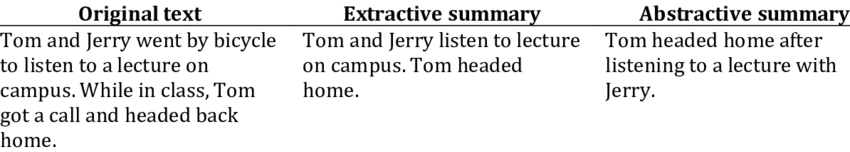
\includegraphics[width=0.8\textwidth]{image/extractive-vs-abstractive.png}
  \caption{Perbandingan pendekatan peringkasan ekstraktif (memilih kalimat penting) dan abstraktif (menghasilkan teks baru) menunjukkan \textit{trade-off} antara \textit{informativeness} dan koherensi}
  \label{fig:extract-abstract}
\end{figure}

\subsection{Peringkasan Multi-Dokumen dan Sintesis Informasi}

Tantangan peringkasan multi-dokumen, yang sangat relevan dengan konteks sintesis lintas tiga grup Telegram, dibahas secara komprehensif oleh \textcite{deyoung2024}. Penelitian mereka mengajukan pertanyaan fundamental: apakah model peringkasan multi-dokumen modern benar-benar dapat mensintesis informasi, atau hanya melakukan agregasi sederhana? Melalui evaluasi terhadap berbagai model dari \textit{fine-tuned transformers} hingga GPT-4, mereka menemukan bahwa sebagian besar model mengalami kesulitan dalam mensintesis informasi yang bertentangan atau berbeda perspektif, dan sangat sensitif terhadap urutan input dokumen. Temuan kritis ini memiliki implikasi langsung bagi desain sistem dalam penelitian ini: sistem harus dirancang dengan mekanisme eksplisit untuk menangani informasi yang mungkin bertentangan antara grup "Cuap Cuap", "Swing Plan", dan "Advanced Group", dan tidak boleh bergantung semata-mata pada kemampuan sintesis implisit LLM.

\textcite{ravaut2024} menyediakan wawasan penting tentang bagaimana LLMs memanfaatkan konteks panjang dalam peringkasan. Penelitian mereka mengungkapkan masalah \textit{position bias}, di mana LLMs cenderung memberikan bobot yang tidak merata terhadap informasi berdasarkan posisinya dalam konteks. Mereka mengevaluasi enam LLMs berbeda pada sepuluh dataset dengan lima metrik evaluasi, menemukan bahwa model cenderung memberikan perhatian berlebihan pada informasi di awal dan akhir konteks, sementara mengabaikan informasi di tengah. Untuk mengatasi masalah ini, mereka memperkenalkan benchmark \textit{MiddleSum} dan mengevaluasi metode hierarkis dan inkremental untuk peringkasan. Temuan ini sangat relevan untuk implementasi Llama 3.1 70B dalam penelitian ini, yang harus memproses konteks panjang (potensial ratusan pesan dalam satu jam). Desain sistem harus mempertimbangkan strategi mitigasi \textit{position bias}, seperti pengelompokan pesan berdasarkan topik sebelum peringkasan atau penggunaan rangkuman inkremental.

\subsection{Peringkasan Percakapan dan Dialog}

\textcite{gliwa2019} memperkenalkan \textit{SAMSum Corpus}, dataset dialog yang dianotasi secara manual untuk peringkasan abstraktif, yang menetapkan bahwa peringkasan percakapan memiliki tantangan unik dibandingkan dengan peringkasan artikel berita. Dialog dan percakapan grup memiliki struktur yang lebih kompleks dengan pergantian pembicara, konteks implisit, referensi anaforik, dan topik yang bercabang. Dataset mereka mendemonstrasikan pentingnya memahami struktur dialog dan dinamika percakapan untuk menghasilkan rangkuman yang akurat dan informatif. Karakteristik ini sangat relevan dengan konteks Telegram, di mana percakapan dapat melibatkan puluhan pembicara dengan topik yang berubah cepat dan sering kali tumpang tindih.

\textcite{tian2024} mengembangkan metodologi peringkasan dialog lebih lanjut dengan mengusulkan pendekatan \textit{Mixture of Experts} (MoE) berbasis LLM. Penelitian mereka memperkenalkan mekanisme \textit{role-oriented routing} yang memilih model atau strategi peringkasan yang sesuai berdasarkan karakteristik informasi percakapan yang berbeda. Pendekatan ini sangat relevan dengan konteks komunitas finansial Telegram yang berjenjang, di mana pesan dari berbagai peran (misalnya, Michael Yeoh sebagai pemimpin komunitas versus anggota biasa) mungkin memerlukan perlakuan berbeda dalam proses peringkasan. Sistem yang dirancang dalam penelitian ini mengadopsi konsep serupa melalui \textit{weighted sentiment analysis} yang memberikan bobot berbeda berdasarkan peran pengirim pesan.

\subsection{Memori Jangka Panjang dalam Sistem Dialog}

Konsep memori jangka panjang dalam sistem percakapan dieksplorasi oleh \textcite{wang2023recursive}, yang mengusulkan metode peringkasan rekursif untuk memungkinkan LLMs mempertahankan konteks percakapan yang panjang. Pendekatan mereka melibatkan pembuatan rangkuman hierarkis dari konteks dialog yang kemudian digunakan untuk menjaga konsistensi dalam percakapan yang berkepanjangan. Konsep ini paralel dengan desain sistem rangkuman per jam dalam penelitian ini, di mana setiap rangkuman per jam dapat dipandang sebagai pembentukan "memori jangka panjang" bagi komunitas. Akumulasi rangkuman per jam ini dapat membentuk representasi terkompresi dari diskusi komunitas yang memungkinkan anggota untuk memahami tren dan perkembangan informasi tanpa harus membaca setiap pesan individual.

\subsection{Metrik Evaluasi untuk Peringkasan}

Evaluasi kualitas rangkuman otomatis merupakan aspek kritis yang dibahas oleh \textcite{zhang2020bertscore}. Mereka memperkenalkan \textit{BERTScore}, metrik evaluasi yang menggunakan \textit{contextual embeddings} dari BERT untuk menghitung kesamaan antara rangkuman yang dihasilkan dan rangkuman referensi, mengatasi keterbatasan metrik berbasis \textit{n-gram} seperti ROUGE yang hanya menghitung kecocokan kata eksak. \textit{BERTScore} mendemonstrasikan korelasi yang lebih baik dengan penilaian manusia karena dapat mengenali parafrase dan kesamaan semantik yang tidak tertangkap oleh metrik tradisional. Penelitian ini mengadopsi \textit{BERTScore} bersama dengan metrik lain untuk evaluasi komprehensif kualitas rangkuman yang dihasilkan sistem.

Namun, \textcite{shen2023} memberikan peringatan penting tentang penggunaan LLMs sebagai evaluator otomatis untuk peringkasan abstraktif. Melalui analisis ekstensif terhadap ChatGPT dan GPT-4 sebagai evaluator, mereka menemukan masalah signifikan dalam stabilitas, reliabilitas, dan ketergantungan pada dimensi evaluasi tertentu. Temuan mereka menunjukkan bahwa evaluasi otomatis berbasis LLM tidak dapat sepenuhnya menggantikan evaluasi manusia, terutama untuk aspek kualitatif seperti koherensi naratif dan relevansi kontekstual. Implikasi bagi penelitian ini adalah perlunya kombinasi antara metrik otomatis (\textit{BERTScore}, ROUGE) dan evaluasi subjektif melalui \textit{feedback} pengguna komunitas untuk mendapatkan penilaian holistik terhadap kualitas rangkuman.

% ==========================================
\section{Analisis Sentimen untuk Media Sosial Finansial}
\label{sec:sentiment-analysis}

Analisis sentimen merupakan komponen esensial dalam memahami dinamika diskusi finansial di media sosial. Bagian ini mengulas perkembangan metodologi analisis sentimen, dengan fokus khusus pada domain finansial dan pemrosesan bahasa Indonesia, serta mengeksplorasi bagaimana sinyal sentimen dari komunitas dapat dimanfaatkan untuk meningkatkan kualitas rangkuman.

\subsection{Model Bahasa untuk Analisis Sentimen Indonesia}

\textcite{wilie2020} memperkenalkan \textit{IndoNLU}, benchmark komprehensif untuk evaluasi pemahaman bahasa Indonesia yang mencakup dua belas tugas termasuk analisis sentimen. Dataset mereka dilatih pada \textit{Indo4B}, korpus bahasa Indonesia dengan empat miliar kata, dan menyediakan model IndoBERT yang mengungguli \textit{multilingual BERT} (mBERT) pada berbagai tugas. Penelitian ini mendemonstrasikan bahwa model bahasa monolingual yang dilatih khusus pada korpus bahasa Indonesia menghasilkan performa superior dibandingkan model multilingual untuk tugas-tugas NLP Indonesia. Kontribusi mereka menetapkan IndoBERT sebagai baseline untuk berbagai aplikasi NLP Indonesia, termasuk implementasi analisis sentimen dalam penelitian ini yang menggunakan \textit{indonesian-roberta-base-emotion-classifier}.

Penelitian oleh \textcite{koto2020} memperkuat temuan ini dengan memperkenalkan \textit{IndoLEM}, benchmark dataset dan model IndoBERT untuk NLP Indonesia. Mereka mendemonstrasikan bahwa \textit{pre-training} pada korpus bahasa Indonesia yang besar (220 juta kata) menghasilkan representasi bahasa yang lebih baik untuk tugas-tugas \textit{downstream} termasuk analisis sentimen, yang mencapai F1-score 84,13\%. Penelitian mereka juga mengeksplorasi \textit{transfer learning} dari model multibahasa, menunjukkan bahwa meskipun model multibahasa dapat memberikan titik awal yang baik, \textit{fine-tuning} pada data Indonesia sangat meningkatkan performa.

\textcite{nugroho2021} menerapkan \textit{fine-tuning} BERT untuk analisis sentimen pada ulasan aplikasi mobile berbahasa Indonesia, konteks yang memiliki kesamaan dengan teks media sosial karena sifatnya yang informal dan sering mengandung bahasa gaul atau singkatan. Penelitian mereka membandingkan model multibahasa dengan model khusus Indonesia, mendemonstrasikan keunggulan \textit{transfer learning} untuk bahasa Indonesia dengan data berlabel terbatas. Temuan mereka sangat relevan dengan penelitian ini, karena pesan Telegram finansial sering kali menggunakan bahasa informal, singkatan, dan istilah khusus yang memerlukan model yang robust terhadap variasi linguistik.

\subsection{Analisis Sentimen Domain Finansial}

\textcite{araci2019} memperkenalkan \textit{FinBERT}, model BERT pertama yang dilatih khusus pada korpus finansial untuk analisis sentimen. Model ini mencapai peningkatan akurasi 15\% dibandingkan BERT umum pada dataset \textit{Financial PhraseBank} dan FiQA. Penelitian ini mendemonstrasikan pentingnya \textit{domain-specific pre-training} untuk teks finansial, yang memiliki karakteristik linguistik unik termasuk terminologi khusus, struktur kalimat formal, dan nuansa sentimen yang berbeda dari domain umum. Konsep sentimen dalam konteks finansial lebih kompleks daripada klasifikasi positif-negatif sederhana; istilah seperti "volatilitas tinggi" dapat memiliki konotasi positif atau negatif tergantung konteks strategi investasi. Temuan ini memotivasi penggunaan model analisis sentimen yang disesuaikan untuk konteks finansial dalam penelitian ini, meskipun disesuaikan untuk bahasa Indonesia.

\textcite{si2014} mengeksplorasi pemanfaatan sentimen media sosial untuk prediksi pergerakan saham dengan mengintegrasikan analisis sentimen Twitter dengan struktur relasi sosial. Penelitian mereka mendemonstrasikan bahwa menggabungkan sentimen dengan informasi jaringan sosial (siapa yang mempengaruhi siapa) secara signifikan meningkatkan akurasi prediksi pergerakan harga saham. Temuan kunci mereka adalah bahwa tidak semua opini memiliki bobot yang sama; pendapat dari individu yang lebih berpengaruh atau kredibel dalam jaringan sosial harus diberi bobot lebih tinggi. Konsep ini memiliki paralel langsung dengan desain sistem dalam penelitian ini, di mana implementasi \textit{weighted sentiment analysis} memberikan bobot berbeda berdasarkan peran pengirim (Michael Yeoh versus anggota biasa), mengakui bahwa tidak semua kontributor dalam komunitas memiliki tingkat pengaruh atau keahlian yang sama.

\subsection{Pemanfaatan Sinyal Komunitas dalam Peringkasan}

\textcite{kano2018} mengusulkan metodologi inovatif untuk memanfaatkan sinyal popularitas dalam media sosial (seperti \textit{votes}, \textit{shares}, \textit{bookmarks}) sebagai label jarak jauh (\textit{distant labels}) untuk peringkasan ekstraktif percakapan online. Penelitian mereka mendemonstrasikan bahwa metrik keterlibatan komunitas dapat berfungsi sebagai indikator kualitas dan relevansi konten, memisahkan kontribusi konten dari faktor kontekstual. Pendekatan ini sangat relevan dengan konteks komunitas Telegram finansial berjenjang dalam penelitian ini, di mana struktur hierarkis (grup "Cuap Cuap", "Swing Plan", "Advanced Group") dan peran pengguna (pemimpin komunitas versus anggota biasa) dapat dimanfaatkan sebagai sinyal implisit tentang pentingnya informasi. Prinsip pemanfaatan sinyal komunitas ini diadopsi secara langsung dalam penelitian ini, di mana "peran pengguna" (misalnya, admin Michael Yeoh versus anggota biasa) digunakan sebagai proksi untuk "popularitas" atau "kredibilitas" informasi, yang kemudian menjadi dasar bagi fitur \textit{weighted sentiment}. Sistem yang dikembangkan mengimplementasikan \textit{weighted sentiment} yang memberikan bobot lebih tinggi pada pesan dari sumber yang lebih kredibel atau berpengaruh dalam komunitas.

\subsection{Klasifikasi Emosi versus Sentimen untuk Investor Ritel}

Pemilihan \textit{indonesian-roberta-base-emotion-classifier} dalam penelitian ini memerlukan justifikasi teoretis, karena berbeda dari pendekatan analisis sentimen finansial konvensional yang fokus pada klasifikasi bullish/bearish atau positif/negatif. Perbedaan fundamental ini didasarkan pada karakteristik unik investor ritel dibandingkan dengan investor institusional atau analis profesional.

Penelitian perilaku keuangan menunjukkan bahwa keputusan investasi ritel sangat dipengaruhi oleh emosi, terutama ketakutan (\textit{fear}) dan keserakahan (\textit{greed}). Berbeda dengan analis profesional yang dilatih untuk membuat keputusan berdasarkan analisis rasional, investor ritel sering kali membuat keputusan yang didorong oleh reaksi emosional terhadap pergerakan pasar atau diskusi komunitas. Dalam konteks komunitas Telegram dengan lebih dari 22.000 anggota yang sebagian besar adalah investor ritel muda, emosi kolektif yang terekspresikan dalam diskusi dapat berfungsi sebagai indikator sentimen pasar yang lebih akurat daripada sekadar klasifikasi positif/negatif.

Model klasifikasi emosi yang digunakan dalam penelitian ini dapat mendeteksi spektrum emosi yang lebih nuansa, termasuk ketakutan, kegembiraan, kemarahan, dan kesedihan. Emosi-emosi ini memberikan sinyal yang lebih kaya tentang psikologi pasar dibandingkan dengan sentimen biner. Misalnya, ekspresi ketakutan tinggi dalam diskusi komunitas dapat mengindikasikan potensi \textit{panic selling}, sementara kegembiraan berlebihan dapat menandakan \textit{euphoria} yang sering kali mendahului koreksi pasar. Pendekatan berbasis emosi ini selaras dengan teori \textit{behavioral finance} yang mengidentifikasi bias psikologis sebagai faktor kunci dalam pengambilan keputusan investasi ritel.

Lebih lanjut, konteks diskusi informal di Telegram lebih cenderung mengekspresikan emosi autentik dibandingkan dengan laporan finansial formal atau analisis profesional. Anggota komunitas sering kali berbagi reaksi emosional mereka terhadap pergerakan harga, keputusan investasi, atau berita pasar dengan cara yang langsung dan tidak tersaring. Klasifikasi emosi dapat menangkap sinyal-sinyal psikologis ini yang hilang dalam analisis sentimen tradisional, memberikan wawasan yang lebih mendalam tentang suasana hati (\textit{mood}) komunitas dan potensi implikasinya terhadap perilaku investasi kolektif.

\begin{figure}[H]
  \centering
  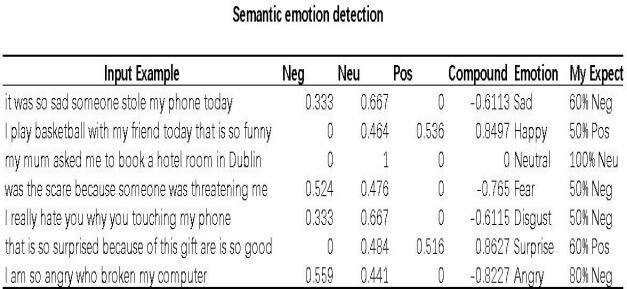
\includegraphics[width=0.75\textwidth]{image/sentiment-analysis-example.jpeg}
  \caption{Contoh klasifikasi emosi pada teks, menunjukkan deteksi berbagai emosi seperti ketakutan, kegembiraan, dan kesedihan yang memberikan sinyal psikologi pasar}
  \label{fig:sentiment-example}
\end{figure}

% ==========================================
\section{\textit{Named Entity Recognition} untuk Teks Finansial Indonesia}
\label{sec:ner}

\textit{Named Entity Recognition} (NER) merupakan tugas fundamental dalam NLP yang bertujuan mengidentifikasi dan mengklasifikasikan entitas bernama dalam teks, seperti nama orang, organisasi, lokasi, dan dalam konteks finansial, nama perusahaan, kode saham (ticker), dan istilah finansial spesifik. Berbeda dengan Section \ref{sec:sentiment-analysis} yang fokus pada ekstraksi sinyal sentimen (\textit{apa yang dirasakan}), NER berfokus pada identifikasi entitas (\textit{siapa} atau \textit{apa yang dibahas}). Kedua komponen ini bersifat komplementer dalam sistem rangkuman: NER mengidentifikasi saham mana yang dibahas, sementara analisis sentimen mengidentifikasi bagaimana komunitas merasakan saham tersebut.

\subsection{NER untuk Bahasa Indonesia}

Sebagaimana telah dibahas dalam Section \ref{sec:sentiment-analysis}, model IndoBERT dari \textcite{koto2020} telah menetapkan fondasi kuat untuk berbagai tugas NLP Indonesia, termasuk NER. Dataset \textit{IndoLEM} yang mereka kembangkan menyediakan benchmark NER bahasa Indonesia yang komprehensif, di mana IndoBERT mencapai performa \textit{state-of-the-art} dengan mengungguli mBERT secara signifikan. Model \textit{cahya/bert-base-indonesian-NER} yang digunakan dalam penelitian ini dibangun di atas arsitektur IndoBERT ini, yang telah di-\textit{fine-tune} khusus untuk tugas ekstraksi entitas.

Penelitian \textcite{khairunnisa2020} mengidentifikasi masalah kritis dalam dataset NER Indonesia yang ada: inkonsistensi anotasi yang dapat menurunkan performa model. Mereka menyediakan dataset yang dianotasi ulang dengan standar yang lebih konsisten dan mengevaluasi berbagai pendekatan \textit{deep learning} termasuk BiLSTM-CRF dengan berbagai jenis \textit{embeddings}. Penelitian mereka menekankan pentingnya kualitas data pelatihan dan konsistensi skema anotasi untuk mencapai performa NER yang optimal. Wawasan ini relevan dengan penelitian ini, terutama dalam konteks adaptasi model NER untuk mengenali entitas finansial spesifik Indonesia yang mungkin tidak terwakili dengan baik dalam dataset NER umum, termasuk penggunaan \textit{whitelist} ticker saham dari Bursa Efek Indonesia untuk meningkatkan akurasi deteksi.

\begin{figure}[H]
  \centering
  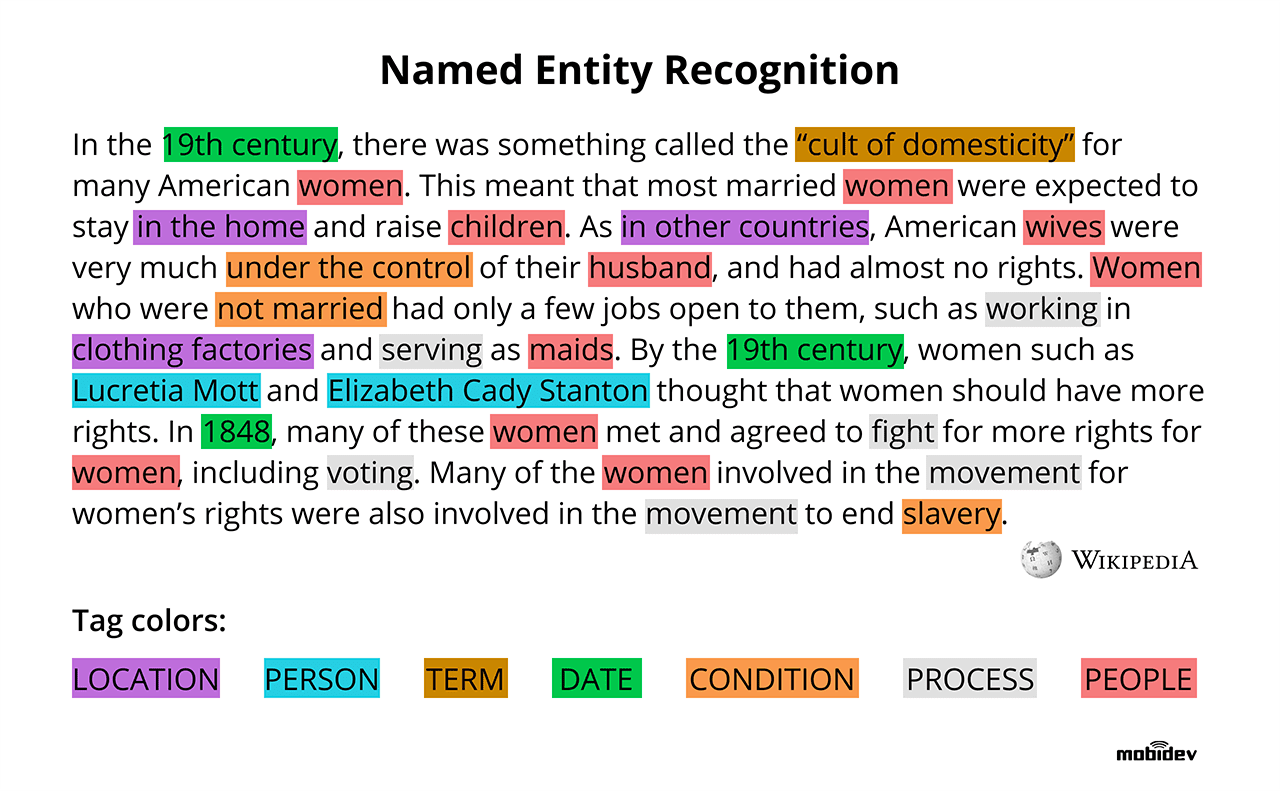
\includegraphics[width=0.85\textwidth]{image/ner-example.png}
  \caption{Contoh \textit{Named Entity Recognition} pada teks, menunjukkan identifikasi entitas seperti nama perusahaan, kode saham, dan lokasi yang diberikan label berbeda}
  \label{fig:ner-example}
\end{figure}

\subsection{NER Domain Finansial}

\textcite{zhang2022finbert} mengembangkan \textit{FinBERT-MRC}, pendekatan NER finansial yang merumuskan tugas ekstraksi entitas sebagai masalah \textit{machine reading comprehension}. Model mereka mencapai F1-score 92,78\% dan 96,80\% pada dataset finansial Tiongkok, mengungguli pendekatan BiLSTM-CRF dan BERT-CRF tradisional. Penelitian ini mendemonstrasikan bahwa NER domain finansial memiliki tantangan unik karena variasi semantik dan leksikal yang spesifik, seperti perbedaan antara nama perusahaan dalam konteks berita versus dokumen formal, atau ambiguitas antara nama organisasi dan produk finansial. Meskipun penelitian mereka fokus pada bahasa Tiongkok, prinsip-prinsip metodologis dapat diadaptasi untuk konteks Indonesia, terutama dalam menangani ambiguitas nama perusahaan versus kode saham.

\textcite{shah2023} menyediakan sumber daya penting untuk NER finansial melalui \textit{FiNER-ORD}, dataset NER finansial \textit{open research} pertama dengan kualitas tinggi. Dataset ini mengatasi variasi semantik dan leksikal yang unik dalam domain finansial dan menyediakan benchmark untuk berbagai model bahasa pra-latih termasuk varian BERT dan LLMs. Penelitian mereka menekankan bahwa entitas finansial sering kali memiliki representasi multipel (misalnya, "Apple Inc.", "Apple", "AAPL") yang harus dikenali sebagai entitas yang sama. Wawasan ini sangat relevan dengan konteks pasar saham Indonesia, di mana perusahaan mungkin dirujuk dengan nama lengkap, nama singkat, atau kode ticker (misalnya, "Bank Central Asia", "BCA", "BBCA").

% ==========================================
\section{\textit{Topic Modeling} dengan BERTopic}
\label{sec:topic-modeling}

\textit{Topic modeling} merupakan teknik untuk mengidentifikasi tema atau topik abstrak dalam kumpulan dokumen. Bagian ini mengulas evolusi metodologi \textit{topic modeling} dari pendekatan statistik tradisional ke pendekatan berbasis \textit{neural embeddings}, dengan fokus khusus pada BERTopic yang digunakan dalam sistem yang dikembangkan.

\subsection{BERTopic: Metodologi dan Keunggulan}

\textcite{grootendorst2022} memperkenalkan BERTopic, metodologi \textit{topic modeling} neural yang menggabungkan model bahasa berbasis \textit{transformer} (BERT), \textit{document embeddings}, \textit{clustering} dengan HDBSCAN, dan prosedur \textit{class-based TF-IDF} (c-TF-IDF) untuk mengekstrak representasi topik yang koheren. Arsitektur BERTopic mengatasi keterbatasan pendekatan tradisional seperti \textit{Latent Dirichlet Allocation} (LDA) dengan memanfaatkan representasi semantik kontekstual dari \textit{transformer models}. Prosedur c-TF-IDF yang diusulkan menghasilkan representasi topik yang lebih interpretatif dibandingkan dengan metode konvensional dengan memperlakukan semua dokumen dalam satu kluster sebagai satu dokumen besar dan membandingkannya dengan dokumen dari kluster lain. Metodologi ini sangat sesuai untuk teks media sosial yang pendek dan informal, karena tidak memerlukan asumsi distribusional yang ketat seperti LDA.

\begin{figure}[H]
  \centering
  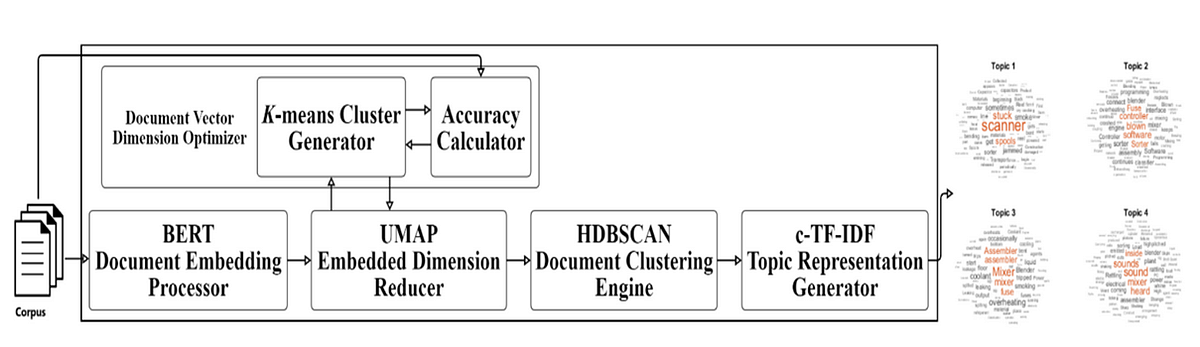
\includegraphics[width=0.85\textwidth]{image/bertopic-workflow.png}
  \caption{Alur kerja BERTopic menunjukkan tahapan dari \textit{document embeddings}, dimensionality reduction dengan UMAP, \textit{clustering} dengan HDBSCAN, hingga ekstraksi representasi topik dengan c-TF-IDF (diadaptasi dari \textcite{grootendorst2022})}
  \label{fig:bertopic-workflow}
\end{figure}

Keunggulan BERTopic untuk teks media sosial divalidasi secara empiris oleh \textcite{egger2022}, yang membandingkan BERTopic dengan LDA, NMF, dan Top2Vec pada dataset 31.800 \textit{tweet} terkait COVID-19 dan perjalanan. Evaluasi mereka mendemonstrasikan superioritas BERTopic untuk teks pendek dan tidak terstruktur, khususnya dalam hal koherensi topik dan interpretabilitas. Metrik evaluasi menunjukkan bahwa BERTopic menghasilkan topik yang lebih koheren dan mudah dipahami dibandingkan dengan metode tradisional, terutama untuk data yang memiliki karakteristik serupa dengan media sosial: panjang dokumen pendek, penggunaan bahasa informal, dan struktur gramatikal yang longgar. Temuan ini memberikan justifikasi kuat untuk pemilihan BERTopic dalam penelitian ini, mengingat pesan Telegram finansial memiliki karakteristik yang sangat mirip dengan \textit{tweet}: pendek, informal, dan sering menggunakan singkatan atau jargon.

\subsection{Perkembangan Terkini dalam \textit{Topic Modeling} Neural}

\textcite{angelov2024} mengembangkan metodologi \textit{topic modeling} lebih lanjut dengan memperkenalkan \textit{Contextual-Top2Vec}, yang menggunakan \textit{contextual token embeddings} dari dokumen untuk menghasilkan topik hierarkis, \textit{topic spans} dalam dokumen, dan label topik berbasis frasa. Penelitian mereka mengusulkan penggunaan \textit{BERTScore} untuk mengevaluasi koherensi dan informativeness topik, mengatasi keterbatasan metrik evaluasi tradisional seperti koherensi berbasis PMI. Model mereka mengungguli pendekatan \textit{state-of-the-art} pada metrik evaluasi komprehensif, mendemonstrasikan bahwa representasi kontekstual dapat meningkatkan kualitas topik yang dihasilkan. Meskipun penelitian ini menggunakan BERTopic sebagai metodologi dasar, wawasan dari \textit{Contextual-Top2Vec} menginformasikan pertimbangan desain, terutama dalam hal evaluasi kualitas topik dan interpretasi hasil \textit{clustering}.

% ==========================================
\section{Telegram sebagai Platform Komunitas}
\label{sec:telegram-platform}

Telegram telah berkembang menjadi platform komunikasi yang dominan untuk komunitas online, terutama di Indonesia. Bagian ini mengulas karakteristik unik Telegram sebagai platform untuk komunitas berskala besar, pola komunikasi yang terjadi di dalamnya, dan implikasi untuk desain sistem analitik dan rangkuman otomatis.

\subsection{Karakteristik dan Dinamika Platform Telegram}

\textcite{nobari2017} menyediakan analisis pionir tentang struktur dan aspek topikal Telegram menggunakan data yang di-\textit{crawl} dari kanal publik. Penelitian mereka mengeksplorasi pola jaringan, klasifikasi pesan (spam/ham), dan arsitektur Telegram sebagai platform \textit{messaging} hibrida yang menggabungkan fitur komunikasi pribadi dan publik. Mereka mengidentifikasi bahwa Telegram memiliki karakteristik unik dibandingkan platform media sosial lain: kombinasi antara privasi komunikasi satu-satu dengan kemampuan penyebaran informasi massal melalui kanal dan grup besar. Struktur ini menciptakan dinamika komunikasi yang berbeda dari platform seperti Twitter atau Facebook, di mana informasi dapat menyebar dengan cepat dalam komunitas tertutup yang besar tanpa eksposur publik yang luas. Pemahaman tentang arsitektur ini penting untuk desain sistem rangkuman yang harus mempertimbangkan privasi komunitas sambil memfasilitasi akses informasi yang efisien.

\textcite{hashemi2019} mengembangkan metodologi untuk mengukur kualitas grup Telegram melalui analisis perilaku pengguna, mengeksplorasi lebih dari 900.000 kanal dan 300.000 \textit{supergroup} berbahasa Persia. Mereka mengusulkan fitur-fitur pengukuran kualitas yang membedakan grup berkualitas tinggi dari grup berkualitas rendah berdasarkan pola aktivitas pengguna, konsistensi partisipasi, dan struktur komunikasi. Penelitian mereka menunjukkan bahwa grup berkualitas tinggi cenderung memiliki partisipasi yang lebih seimbang, topik diskusi yang lebih fokus, dan tingkat spam yang lebih rendah. Temuan ini relevan dengan konteks komunitas Michael Yeoh yang memiliki struktur berjenjang, di mana grup "Advanced" diasumsikan memiliki kualitas diskusi yang lebih tinggi dibandingkan grup "Cuap Cuap" umum. Sistem rangkuman harus dirancang dengan mempertimbangkan perbedaan kualitas dan karakteristik diskusi antar grup.

\subsection{Analisis Skala Besar Komunitas Telegram}

\textcite{lamorgia2024} menyediakan dataset Telegram terbesar hingga saat ini dengan 120.979 kanal dan lebih dari 400 juta pesan, bersama dengan infrastruktur untuk pengumpulan dan analisis data skala besar. Penelitian mereka menyediakan alat dan metodologi untuk penelitian komunitas Telegram yang mencakup analisis dinamika komunitas, propagasi konten, dan pola komunikasi tingkat platform. Kontribusi mereka mendemonstrasikan bahwa Telegram telah berkembang menjadi ekosistem informasi yang kompleks dengan dinamika komunitas yang beragam. Skala dataset ini memberikan konteks untuk memahami bahwa komunitas finansial dengan 22.000+ anggota seperti yang diteliti dalam penelitian ini merupakan bagian dari fenomena komunikasi online yang lebih luas, di mana platform seperti Telegram telah menjadi infrastruktur kritis untuk pertukaran informasi dalam komunitas tematik berskala besar.

Penelitian terbaru oleh \textcite{perlo2025} menyediakan analisis per-topik pertama dari grup Telegram, mengeksplorasi 51 juta pesan dari 669 grup di berbagai topik termasuk Pendidikan, Politik, dan Cryptocurrency. Penelitian mereka menganalisis pola aktivitas pengguna, kehadiran bot, dan berbagi media, serta menyediakan alat \textit{open-source} untuk pengumpulan pesan otomatis. Temuan kunci mereka adalah bahwa grup dengan topik berbeda menunjukkan pola komunikasi yang sangat berbeda dalam hal volume pesan, distribusi waktu aktivitas, dan tipe konten yang dibagikan. Khususnya untuk kategori Cryptocurrency, yang memiliki kesamaan dengan komunitas finansial yang diteliti, mereka menemukan tingkat aktivitas yang sangat tinggi dengan puncak aktivitas yang berkorelasi dengan jam perdagangan pasar. Temuan ini memvalidasi desain sistem rangkuman per jam dalam penelitian ini, karena pola aktivitas temporal yang kuat mengindikasikan bahwa rangkuman periodik sesuai dengan ritme alami diskusi komunitas.

% ==========================================
\section{Arsitektur Pemrosesan Data \textit{Real-Time}}
\label{sec:realtime-architecture}

Implementasi sistem rangkuman otomatis untuk komunitas Telegram yang aktif memerlukan arsitektur pemrosesan data yang dapat menangani aliran pesan secara \textit{real-time} atau \textit{near-real-time}. Bagian ini mengulas pendekatan arsitektural untuk pemrosesan \textit{stream} teks dengan NLP, pola \textit{event-driven architecture}, dan pertimbangan desain untuk sistem yang responsif dan \textit{scalable}.

\subsection{\textit{Pipeline} NLP untuk Pemrosesan \textit{Stream} Teks}

\textcite{hamidi2021} mengusulkan arsitektur \textit{pipeline} NLP yang dinamis dan terdistribusi untuk pemrosesan \textit{stream} teks \textit{real-time}. Penelitian mereka menggunakan Apache Storm dan Apache Kafka untuk menerapkan tugas-tugas NLP pada aliran data tekstual, memungkinkan pengembang untuk menginjeksi modul NLP melalui berbagai bahasa pemrograman dan mendukung sumber data multipel. Arsitektur mereka mendemonstrasikan bagaimana komponen NLP yang berbeda (tokenisasi, \textit{part-of-speech tagging}, \textit{named entity recognition}, analisis sentimen) dapat dikomposisikan dalam \textit{pipeline} yang dapat di-\textit{scale} secara horizontal. Prinsip-prinsip desain ini relevan dengan penelitian ini, di mana sistem harus mengintegrasikan beberapa komponen NLP (analisis sentimen, NER, \textit{topic modeling}, generasi rangkuman) dalam arsitektur yang koheren dan dapat diperluas.

\textcite{isah2019} menyediakan survei komprehensif tentang \textit{framework} pemrosesan \textit{stream} data terdistribusi, termasuk Apache Storm, Spark Streaming, Apache Flink, dan Kafka Streams. Penelitian mereka membandingkan model pemrosesan, karakteristik operasional, dan pola arsitektural dari berbagai \textit{framework}, memberikan taksonomi yang membantu dalam pemilihan teknologi yang sesuai untuk kasus penggunaan spesifik. Untuk konteks komunitas Telegram dengan volume pesan yang tinggi namun tidak ekstrem (ratusan hingga ribuan pesan per jam), mereka mengidentifikasi bahwa pendekatan \textit{micro-batch processing} dengan Kafka atau arsitektur berbasis \textit{event} yang lebih sederhana dapat memberikan keseimbangan optimal antara latensi, throughput, dan kompleksitas implementasi. Wawasan ini menginformasikan desain sistem dalam penelitian ini, yang mengadopsi arsitektur berbasis \textit{event} dengan penjadwalan periodik daripada pemrosesan \textit{stream} kontinu, sesuai dengan kebutuhan rangkuman per jam.

\subsection{Arsitektur Berbasis \textit{Event} dan Performa}

\textcite{rubert2023} menyediakan bukti empiris tentang dampak \textit{event-driven architecture} (EDA) terhadap performa melalui studi eksploratif yang membandingkan arsitektur berbasis \textit{event} dengan arsitektur monolitik. Penelitian mereka mengukur penggunaan CPU, memori, waktu respons, \textit{throughput}, dan paket jaringan, mendemonstrasikan bahwa EDA dapat memberikan keunggulan signifikan dalam \textit{scalability} dan responsivitas, terutama untuk sistem yang menangani beban kerja yang bervariasi dan tidak dapat diprediksi. Temuan mereka menunjukkan bahwa EDA sangat cocok untuk skenario di mana komponen sistem perlu berkomunikasi secara asinkron dan dapat di-\textit{scale} secara independen. Konteks komunitas Telegram finansial, di mana volume pesan bervariasi drastis sepanjang hari (tinggi selama jam perdagangan, rendah di malam hari), sangat sesuai dengan karakteristik ini. Sistem yang dikembangkan dalam penelitian ini mengadopsi prinsip EDA dengan pemisahan antara komponen pengumpulan pesan, pemrosesan NLP, dan generasi rangkuman, memungkinkan setiap komponen untuk beroperasi secara independen dan di-\textit{scale} sesuai kebutuhan.

\subsection{Pertimbangan \textit{Micro-batching} dan Frekuensi Data}

Meskipun pemrosesan \textit{stream} murni memberikan latensi terendah, penelitian menunjukkan bahwa pendekatan \textit{micro-batching} sering kali lebih praktis untuk banyak aplikasi NLP. Konsep rangkuman per jam dalam penelitian ini dapat dipandang sebagai bentuk \textit{macro-batching}, di mana pesan dikumpulkan selama satu jam sebelum diproses sebagai satu \textit{batch}. Pendekatan ini memberikan beberapa keuntungan: (1) memungkinkan agregasi konteks yang lebih kaya untuk tugas-tugas seperti \textit{topic modeling} yang memerlukan pandangan holistik terhadap data, (2) mengurangi beban komputasi dengan menghindari pemrosesan setiap pesan individual secara \textit{real-time}, dan (3) sesuai dengan ritme natural konsumsi informasi pengguna, yang jarang memerlukan pembaruan lebih sering dari setiap jam untuk analisis tren komunitas.

\subsection{Tantangan Inferensi LLM dalam Sistem \textit{Real-Time}}

Bottleneck arsitektural yang paling signifikan dalam sistem rangkuman otomatis berbasis LLM adalah latensi inferensi model bahasa besar. Tidak seperti komponen NLP tradisional seperti tokenisasi atau \textit{named entity recognition} yang dapat dieksekusi dalam milidetik, generasi teks dengan LLM skala besar (puluhan hingga ratusan miliar parameter) dapat memerlukan waktu detik hingga menit untuk satu panggilan inferensi, tergantung pada panjang konteks input dan panjang output yang dihasilkan. Tantangan ini menjadi kritis dalam konteks sistem rangkuman per jam, di mana seluruh \textit{pipeline} pemrosesan harus selesai dalam jendela waktu yang terbatas (idealnya kurang dari 5-10 menit dari akhir periode pengumpulan data) untuk menjaga relevansi temporal rangkuman.

Penelitian terkini menunjukkan bahwa kecepatan inferensi LLM sangat dipengaruhi oleh tiga faktor utama: (1) ukuran model (jumlah parameter), (2) panjang konteks input, dan (3) infrastruktur komputasi yang digunakan (CPU, GPU, atau akselerator khusus seperti TPU). Untuk konteks rangkuman komunitas Telegram dengan potensi ratusan pesan per jam, panjang konteks input dapat dengan mudah mencapai puluhan ribu \textit{token}, yang secara signifikan meningkatkan waktu inferensi pada infrastruktur standar. Lebih lanjut, model yang lebih besar seperti Llama 3.1 70B, meskipun memberikan kualitas output superior dibandingkan model yang lebih kecil, memerlukan sumber daya komputasi yang substansial dan dapat mengalami latensi yang tidak dapat diterima pada infrastruktur konvensional.

Pemilihan Groq API dengan model Llama 3.1 70B dalam penelitian ini merupakan solusi arsitektural yang dirancang khusus untuk mengatasi bottleneck inferensi LLM ini. Groq menggunakan \textit{Language Processing Unit} (LPU), arsitektur akselerator khusus yang dirancang untuk inferensi LLM dengan kecepatan ekstrem. Platform Groq telah mendemonstrasikan kemampuan untuk menghasilkan ratusan hingga ribuan \textit{tokens per second}, secara signifikan melampaui solusi berbasis GPU tradisional. Kecepatan inferensi yang tinggi ini adalah faktor pendukung (\textit{enabler}) teknis yang krusial yang memungkinkan implementasi rangkuman per jam yang praktis; tanpa throughput inferensi yang tinggi, sistem akan mengalami akumulasi \textit{backlog} dan keterlambatan yang tidak dapat diterima, merusak nilai temporal dari rangkuman yang dihasilkan.

Selain itu, penggunaan \textit{API} cloud seperti Groq menghilangkan kompleksitas operasional dalam mengelola infrastruktur inferensi LLM lokal, termasuk manajemen GPU, optimasi \textit{batch size}, dan penjadwalan sumber daya. Pendekatan ini memungkinkan sistem untuk fokus pada logika bisnis dan integrasi komponen NLP, sementara kebutuhan komputasi intensif untuk inferensi LLM di-\textit{offload} ke platform yang dioptimalkan. Arsitektur ini mencerminkan prinsip \textit{separation of concerns} dalam desain sistem terdistribusi, di mana setiap komponen (pengumpulan data, pemrosesan NLP, inferensi LLM) diimplementasikan menggunakan teknologi yang paling sesuai untuk karakteristik komputasinya.

% ==========================================
\section{Peringkasan untuk Media Sosial dan Percakapan Online}
\label{sec:social-media-summarization}

Peringkasan konten media sosial memiliki tantangan unik dibandingkan dengan peringkasan dokumen formal atau artikel berita, termasuk bahasa informal, topik yang bercabang, dan struktur percakapan yang kompleks. Bagian ini mengulas penelitian tentang peringkasan media sosial, khususnya Reddit dan forum diskusi online, yang memiliki karakteristik serupa dengan komunitas Telegram. Berbeda dengan Section \ref{sec:sentiment-analysis} yang fokus pada ekstraksi sinyal sentimen individual, bagian ini membahas sintesis informasi kolektif dari percakapan \textit{multi-speaker}.

\subsection{Peringkasan Percakapan dengan \textit{Argument Mining}}

\textcite{fabbri2021} memperkenalkan \textit{ConvoSumm}, benchmark peringkasan percakapan yang mencakup empat dataset dari berbagai bentuk percakapan online: komentar berita, forum diskusi, forum Q\&A komunitas, dan \textit{thread} email. Penelitian mereka menggunakan \textit{framework} \textit{issues-viewpoints-assertions} yang menginkorporasikan \textit{argument mining} melalui konstruksi graf untuk memodelkan struktur percakapan. Pendekatan ini mengakui bahwa percakapan online sering kali melibatkan pertukaran pandangan yang kompleks dengan argumen pendukung, yang memerlukan pemahaman struktural lebih mendalam daripada sekadar ekstraksi kalimat penting. Kontribusi metodologis mereka relevan dengan penelitian ini karena diskusi finansial di Telegram sering kali mengandung perdebatan antara strategi investasi berbeda, analisis yang bertentangan, atau perspektif pasar yang beragam. Sistem rangkuman yang efektif harus dapat mensintesis pandangan-pandangan yang berbeda ini daripada hanya mengekstrak opini dominan.

\subsection{Peringkasan Percakapan \textit{Multi-speaker}}

Kompleksitas percakapan \textit{multi-speaker} dibahas secara komprehensif oleh \textcite{chen2021}, yang mengusulkan pendekatan yang sadar struktur (\textit{structure-aware}) untuk peringkasan percakapan abstraktif. Penelitian mereka memodelkan relasi wacana dan \textit{action triples} ("siapa-melakukan-apa") menggunakan graf terstruktur untuk menangkap karakteristik kompleks interaksi manusia-manusia di media sosial. Mereka mengimplementasikan mekanisme \textit{decoding} multi-granularitas yang dapat menghasilkan rangkuman pada tingkat abstraksi berbeda. Pendekatan ini sangat relevan dengan konteks komunitas Telegram berjenjang, di mana percakapan melibatkan puluhan hingga ratusan partisipan dengan peran dan tingkat keahlian yang berbeda. Sistem harus dapat mengenali struktur interaksi (misalnya, pertanyaan-jawaban, klaim-dukungan, analisis-counter-analisis) untuk menghasilkan rangkuman yang koheren dan informatif.

\subsection{Peringkasan Ekstrim untuk Konten Media Sosial}

\textcite{sotudeh2021} memperkenalkan dataset TLDR9+ dengan lebih dari 9 juta \textit{instance} pelatihan dari Reddit untuk peringkasan ekstrim (rangkuman satu kalimat). Penelitian mereka mengatasi agregasi konten media sosial skala besar dan mencakup subset berkualitas tinggi (TLDRHQ) melalui anotasi manusia. Mereka mendemonstrasikan bahwa peringkasan ekstrim, yang menghasilkan rangkuman sangat singkat dengan tingkat kompresi dan abstraksi tinggi, dapat efektif untuk konten media sosial yang cenderung verbose dan mengandung banyak informasi redundan. Konsep peringkasan ekstrim ini relevan dengan kebutuhan komunitas Telegram finansial, di mana anggota mungkin memerlukan "snapshot" cepat dari diskusi komunitas tanpa membaca rangkuman panjang. Sistem yang dikembangkan dalam penelitian ini dapat mengadaptasi prinsip ini dengan menyediakan "headline" atau "key takeaway" di awal setiap rangkuman per jam sebelum menyajikan detail yang lebih mendalam.

% ==========================================
\section{Kesenjangan Penelitian dan Kontribusi}
\label{sec:research-gaps}

Tinjauan literatur komprehensif di atas mengidentifikasi beberapa kesenjangan penelitian kritis yang ditangani oleh penelitian ini. Pertama, tidak ada penelitian yang mengintegrasikan NLP bahasa Indonesia (khususnya model berbasis RoBERTa dan BERT) dengan analisis domain finansial untuk konteks media sosial. Sebagian besar penelitian analisis sentimen finansial fokus pada bahasa Inggris atau Tiongkok, sementara penelitian NLP Indonesia cenderung menggunakan domain umum atau ulasan produk. Penelitian ini menjembatani kesenjangan ini dengan mengembangkan sistem yang mengintegrasikan \textit{indonesian-roberta-base-emotion-classifier} dan \textit{bert-base-indonesian-NER} untuk analisis teks finansial Indonesia dalam konteks media sosial.

Kedua, meskipun terdapat penelitian ekstensif tentang komunitas Telegram dan peringkasan media sosial secara terpisah, sangat sedikit penelitian yang menangani sistem peringkasan otomatis khusus untuk aplikasi bot Telegram. Penelitian tentang bot Telegram cenderung fokus pada interaksi percakapan sederhana atau otomasi tugas administratif, bukan pada sintesis intelijen informasi yang kompleks. Penelitian ini memberikan kontribusi dengan mendemonstrasikan implementasi praktis sistem peringkasan otomatis yang diintegrasikan dengan Telegram Bot API untuk penyampaian rangkuman periodik.

Ketiga, penelitian tentang \textit{pipeline} NLP \textit{real-time} yang mengintegrasikan multiple model (analisis sentimen, NER, \textit{topic modeling}, generasi rangkuman dengan LLM) dalam arsitektur \textit{event-driven} untuk platform \textit{messaging} masih terbatas. Sebagian besar penelitian mengevaluasi model-model ini secara terpisah atau dalam konteks dataset benchmark offline. Penelitian ini memberikan kontribusi metodologis dengan mendemonstrasikan integrasi empat komponen NLP berbeda dalam sistem yang koheren dan operasional.

Keempat, tidak ada penelitian yang menangani aliran informasi hierarkis dan sintesis lintas grup dalam komunitas berjenjang. Sebagian besar penelitian peringkasan media sosial mengasumsikan satu sumber data atau agregasi horizontal dari multiple sumber yang setara. Penelitian ini menangani skenario unik di mana informasi mengalir melalui struktur hierarkis (grup Cuap Cuap, Swing Plan, Advanced) dengan karakteristik diskusi yang berbeda, dan sistem harus mensintesis informasi lintas tingkat hierarki ini.

Kelima, pendekatan rangkuman per jam untuk diskusi finansial dengan \textit{weighted sentiment} berbasis peran pengguna merupakan kontribusi novel. Sementara penelitian sebelumnya mengeksplorasi pemanfaatan sinyal popularitas atau metrik keterlibatan, penelitian ini mengimplementasikan \textit{weighting} eksplisit berdasarkan struktur peran komunitas yang mencerminkan kredibilitas dan pengaruh relatif kontributor dalam ekosistem informasi finansial.

Secara keseluruhan, penelitian ini mengintegrasikan teori \textit{information overload} dan \textit{cognitive load}, metodologi NLP terkini untuk bahasa Indonesia dan domain finansial, arsitektur pemrosesan \textit{event-driven}, dan pemahaman tentang dinamika komunitas Telegram untuk mengembangkan solusi holistik yang mengatasi tantangan praktis dalam komunitas finansial Indonesia. Kontribusi utama penelitian ini terletak pada demonstrasi bahwa sistem otomatis berbasis \textit{AI} dapat secara efektif mereduksi \textit{information overload} dalam komunitas online berskala besar melalui sintesis intelijen multi-sumber, lintas-grup (\textit{cross-group}), dan hierarkis yang disesuaikan dengan konteks spesifik ekosistem informasi komunitas.

% ============================================================================================
% BAB III ANALISIS MASALAH
% Pembagian subbab tidak rigid dan dapat bervariasi. Bab ini minimal berisi analisis kebutuhan
% fungsional dan nonfungsional, analisis berbagai alternatif solusi yang dapat ditawarkan, dan
% metode pemilihan solusi yang diusulkan.
% ============================================================================================
\chapter{ANALISIS MASALAH}
\label{chap:analisis-masalah}

Bab ini menyajikan analisis mendalam terhadap kondisi sistem komunitas Telegram Michael Yeoh saat ini, identifikasi masalah spesifik yang dihadapi, analisis kebutuhan sistem rangkuman otomatis, serta evaluasi berbagai alternatif solusi dengan justifikasi pemilihan pendekatan yang diusulkan. Analisis ini menjadi fondasi untuk desain konsep solusi yang akan diuraikan pada Bab \ref{chap:desain-konsep-solusi}.

% ==========================================
\section{Analisis Kondisi Saat Ini}
\label{sec:kondisi-saat-ini}

\subsection{Model Konseptual Komunitas Telegram Eksisting}

Komunitas investasi saham Indonesia Michael Yeoh di Telegram merupakan ekosistem informasi finansial berskala besar dengan struktur hierarkis empat tingkat yang dirancang untuk menyediakan nilai berbeda pada setiap level keanggotaan. Gambar \ref{fig:current-system} mengilustrasikan arsitektur sistem komunikasi komunitas saat ini beserta aliran informasi antar komponen.

\begin{figure}[H]
  \centering
  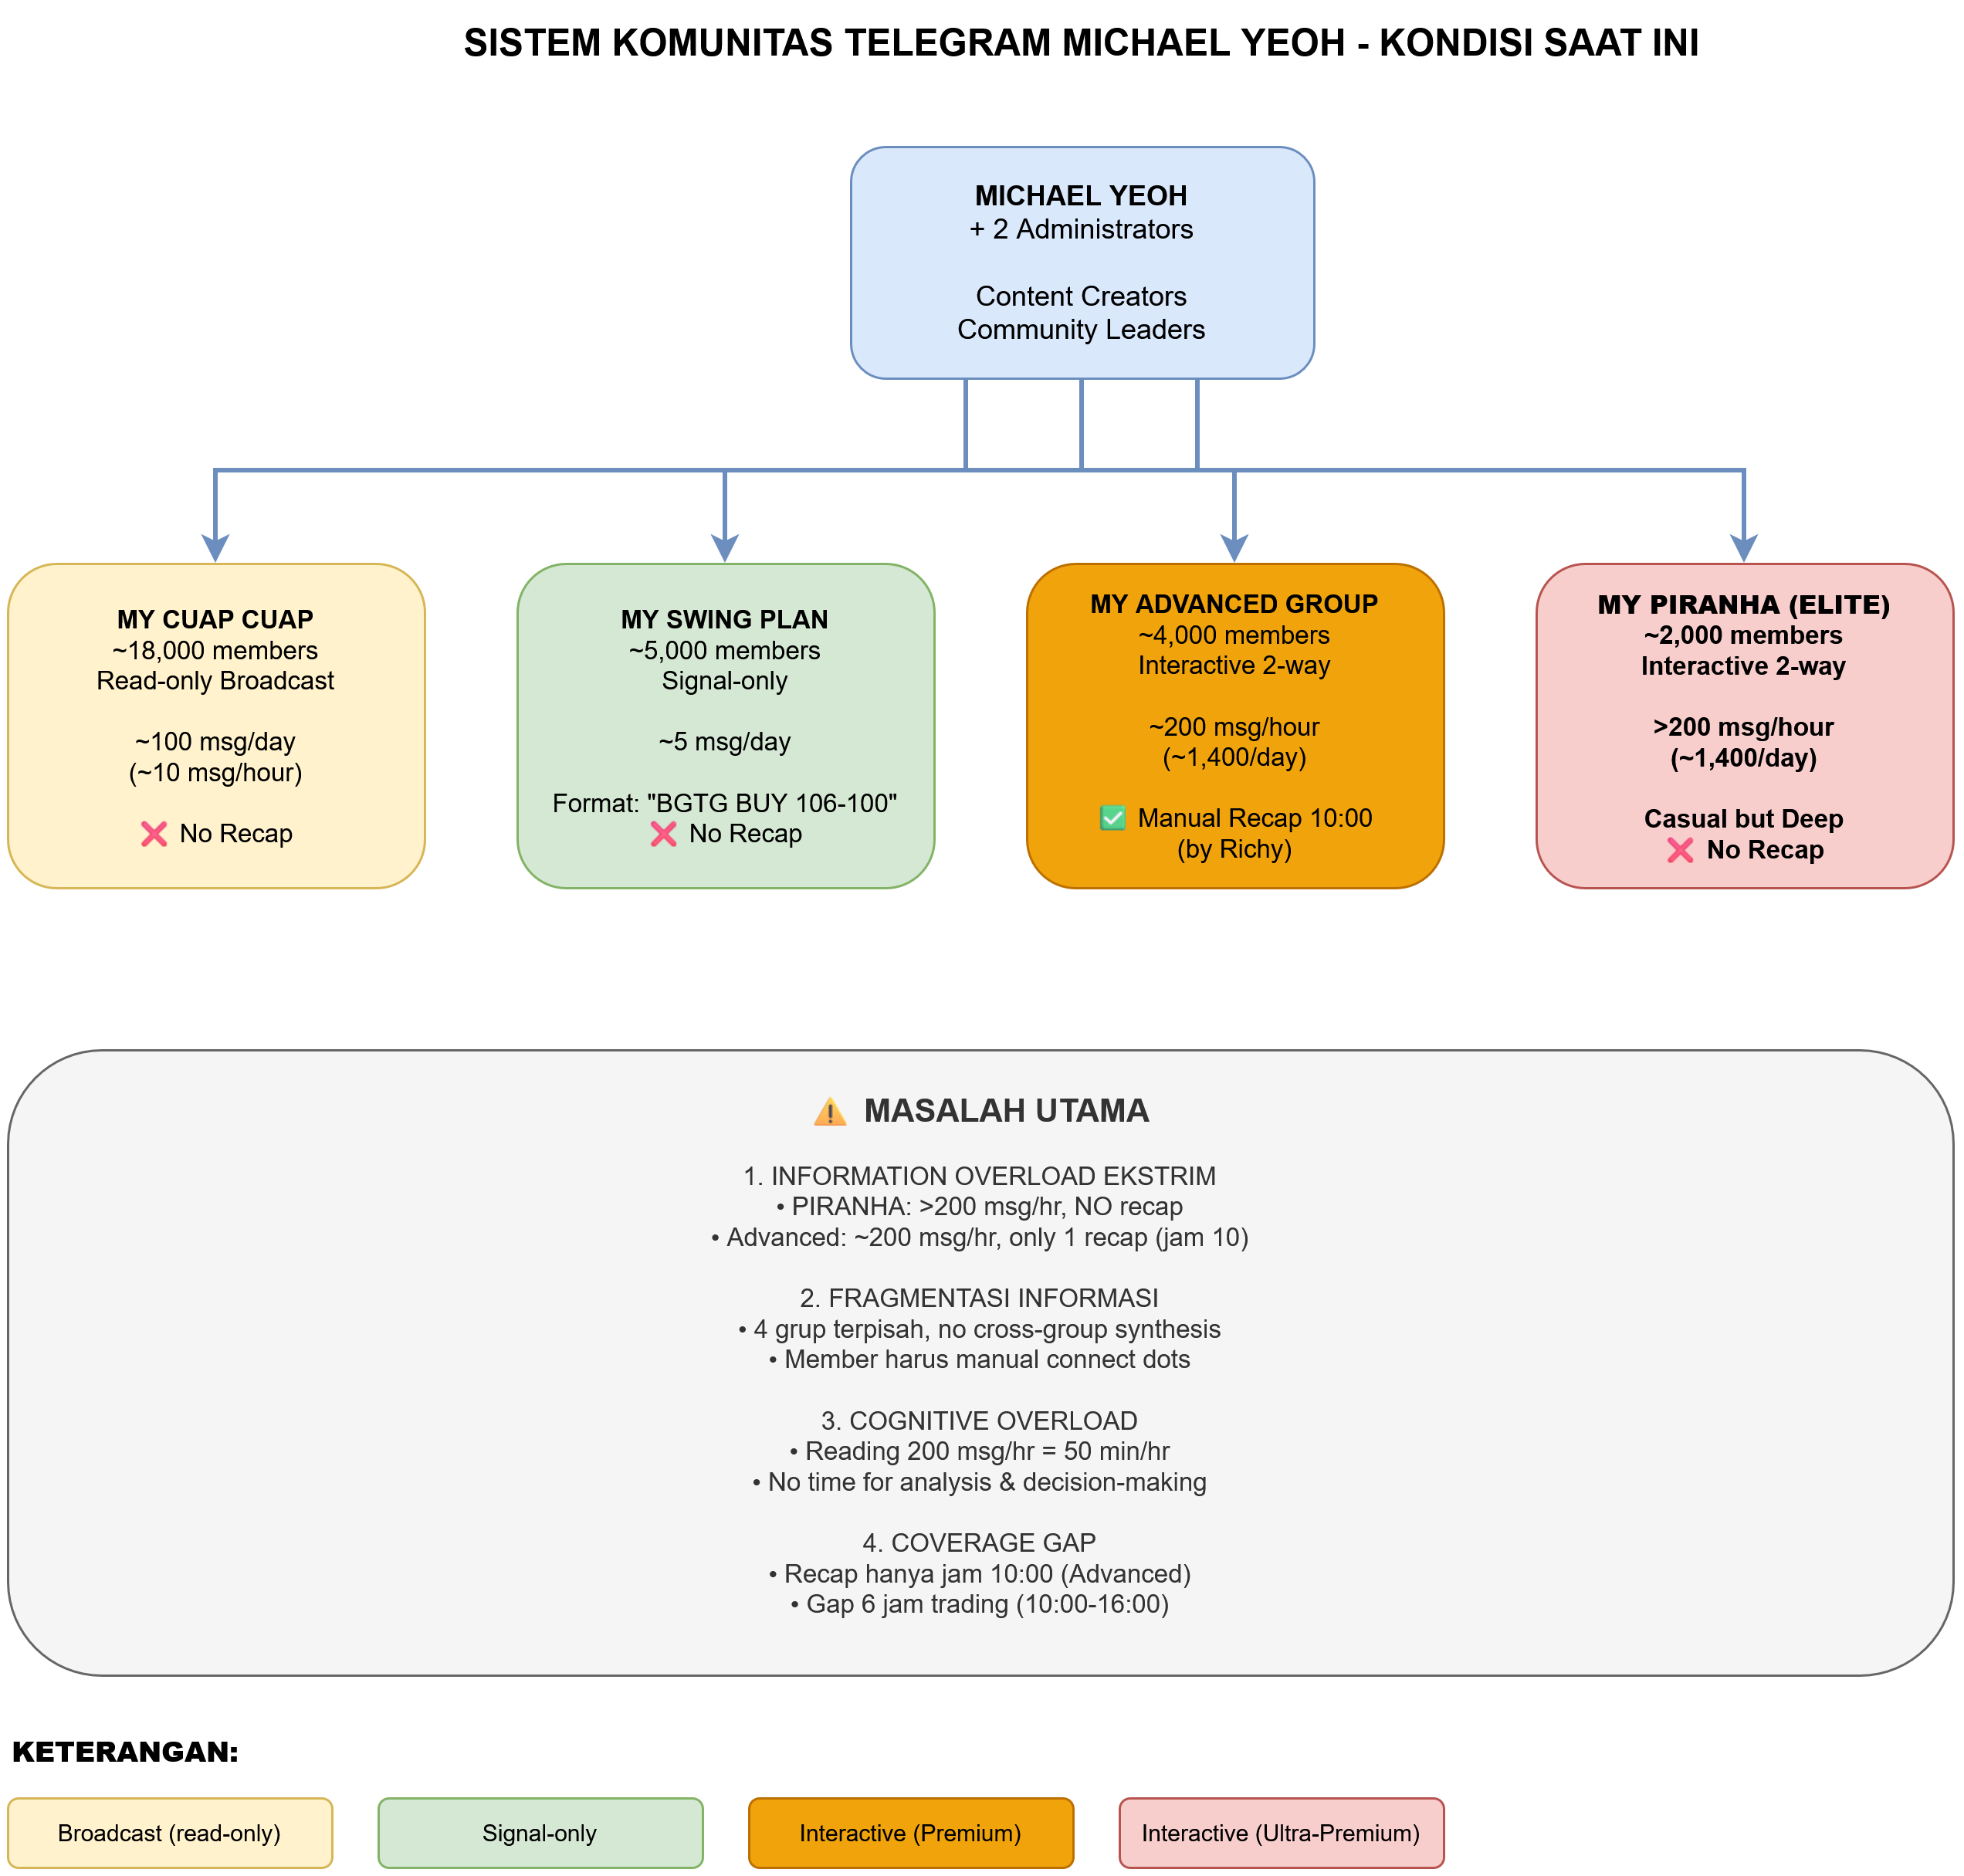
\includegraphics[width=0.9\textwidth]{image/current-state-diagram.png}
  \caption{Model konseptual sistem komunikasi komunitas Telegram Michael Yeoh saat ini}
  \label{fig:current-system}
\end{figure}

Struktur hierarkis komunitas terdiri dari empat grup dengan karakteristik berbeda yang dapat dilihat pada Tabel \ref{tab:group-characteristics}. Setiap grup memiliki fungsi spesifik dalam ekosistem informasi komunitas, dengan kompleksitas komunikasi yang meningkat seiring level hierarki.

\begin{table}[H]
\centering
\caption{Karakteristik grup dalam komunitas Telegram Michael Yeoh}
\label{tab:group-characteristics}
\begin{tabular}{|p{3cm}|p{2.5cm}|p{2.5cm}|p{3cm}|p{2.5cm}|}
\hline
\textbf{Aspek} & \textbf{Cuap Cuap} & \textbf{Swing Plan} & \textbf{Advanced} & \textbf{PIRANHA} \\
\hline
Jumlah Member & ~18.000 & ~5.000 & ~4.000 & ~2.000 \\
\hline
Tipe Komunikasi & Broadcast (\textit{read-only}) & Signal-only & Interaktif 2-arah & Interaktif 2-arah \\
\hline
Volume Pesan & ~100 msg/hari (~10/jam) & ~5 msg/hari & ~200 msg/jam & >200 msg/jam \\
\hline
Konten Utama & Edukasi umum, berita pasar & Sinyal beli/jual terstruktur & Diskusi analisis teknikal & Debat strategi expert \\
\hline
\textit{Recap} Manual & Tidak ada & Tidak ada & 1× per hari (jam 10:00) & Tidak ada \\
\hline
Tingkat Masalah & Rendah & Minimal & Tinggi & Sangat Tinggi \\
\hline
\end{tabular}
\end{table}

Setiap grup dalam hierarki komunitas memiliki peran dan dinamika komunikasi yang berbeda. Grup MY Cuap Cuap berfungsi sebagai kanal informasi umum dengan mode \textit{read-only}, di mana hanya administrator dan Michael Yeoh yang dapat mengirim pesan. Konten utama meliputi edukasi pasar saham, analisis makroekonomi, dan pengumuman penting. Dengan volume sekitar 100 pesan per hari atau rata-rata 10 pesan per jam, grup ini memiliki tingkat \textit{information overload} yang relatif rendah.

Grup MY Swing Plan merupakan kanal khusus untuk distribusi sinyal \textit{trading} dengan format terstruktur seperti "BGTG BUY 106-100 SL 98 porsi 5\%". Volume pesan sangat rendah (~5 pesan per hari) karena sifatnya yang spesifik dan terarah. Grup ini tidak mengalami masalah \textit{information overload}, namun menjadi bagian penting dari ekosistem informasi yang perlu disintesis dengan diskusi di grup lain untuk memberikan konteks komprehensif.

Grup MY Advanced Group adalah grup premium pertama dengan komunikasi interaktif dua arah, di mana sekitar 4.000 anggota dapat berdiskusi secara langsung. Volume pesan mencapai sekitar 200 pesan per jam selama jam perdagangan aktif (09:00-16:00), menghasilkan total sekitar 1.400 pesan per hari. Grup ini memiliki satu rangkuman manual yang dibuat oleh asisten bernama Richy Matthew Ashari setiap hari pada jam 10:00 pagi. Rangkuman manual ini mencakup kondisi pasar dan pergerakan saham-saham prioritas (\textit{PP stocks}) dengan format yang mencantumkan level support, resistance, dan analisis kekuatan saham. Namun, rangkuman ini hanya mencakup satu jam pertama perdagangan (09:00-10:00), meninggalkan gap informasi selama enam jam perdagangan berikutnya (10:00-16:00).

Grup MY PIRANHA merupakan grup ultra-premium dengan 2.000 anggota elite dan mengalami volume pesan tertinggi, melebihi 200 pesan per jam, menghasilkan lebih dari 1.400 pesan per hari. Berbeda dengan Advanced Group, PIRANHA tidak memiliki rangkuman manual sama sekali. Diskusi di grup ini cenderung lebih kasual dalam gaya komunikasi namun sangat mendalam secara konten, dengan debat strategi investasi antar investor berpengalaman. Paradoks "kasual namun \textit{high-volume}" ini menciptakan tantangan ekstraksi sinyal yang unik, karena informasi penting sering tersembunyi dalam percakapan informal yang memerlukan pemahaman konteks mendalam.

Aliran informasi dalam ekosistem komunitas bersifat hierarkis dan fragmentasi. Michael Yeoh dan dua administrator lainnya dapat memposting di semua grup, menciptakan aliran informasi vertikal dari puncak hierarki. Namun, anggota di level berbeda tidak dapat mengakses informasi di grup yang lebih tinggi kecuali mereka menjadi anggota grup tersebut. Hal ini menciptakan fragmentasi informasi di mana analisis makro di Cuap Cuap, sinyal konkret di Swing Plan, diskusi implementasi di Advanced, dan debat strategi di PIRANHA terpisah satu sama lain. Anggota yang merupakan bagian dari multiple grup harus secara manual melakukan sintesis informasi lintas grup, yang memerlukan waktu dan kemampuan analisis yang signifikan.

\subsection{Identifikasi Masalah Sistem Saat Ini}

Berdasarkan analisis terhadap model konseptual sistem saat ini, terdapat tiga kategori masalah utama yang menjadi fokus penelitian ini: \textit{information overload} dengan intensitas ekstrim di grup premium, fragmentasi informasi lintas struktur hierarkis, dan keterbatasan kognitif anggota dalam memproses volume informasi tinggi.

\subsubsection{\textit{Information Overload} Ekstrim di Grup PIRANHA}

Grup PIRANHA mengalami tingkat \textit{information overload} paling parah dalam ekosistem komunitas. Dengan volume melebihi 200 pesan per jam selama jam perdagangan (09:00-16:00), grup ini menghasilkan lebih dari 1.400 pesan per hari. Tidak adanya mekanisme rangkuman otomatis atau manual membuat anggota dihadapkan pada dua pilihan yang sama-sama suboptimal: (1) memantau diskusi secara \textit{real-time} yang memerlukan perhatian konstan selama tujuh jam perdagangan, atau (2) melakukan \textit{catch-up} dengan membaca ratusan pesan secara retrospektif, yang berisiko kehilangan konteks temporal dan relevansi diskusi.

Karakteristik unik dari diskusi PIRANHA yang kasual namun mendalam memperburuk masalah ini. Tidak seperti diskusi terstruktur di grup lain, informasi kritis di PIRANHA sering tersembunyi dalam percakapan informal tanpa penanda eksplisit seperti format sinyal trading atau header topik. Ekstraksi sinyal dari diskusi kasual memerlukan pemahaman konteks yang dalam, yang sulit dilakukan ketika anggota harus memproses volume pesan yang sangat tinggi dalam waktu terbatas.

Dampak kuantitatif dari masalah ini dapat diestimasi menggunakan kerangka \textit{Cognitive Load Theory}. Jika diasumsikan rata-rata waktu baca dan pemahaman per pesan adalah 15 detik, maka untuk membaca 200 pesan memerlukan 50 menit, mendekati satu jam penuh. Selama jam perdagangan yang berlangsung selama tujuh jam, anggota yang mencoba membaca semua pesan akan menghabiskan hampir seluruh waktu mereka hanya untuk konsumsi informasi, tanpa waktu untuk analisis dan pengambilan keputusan. Situasi ini jelas tidak sustainable dan bertentangan dengan tujuan komunitas untuk memfasilitasi pengambilan keputusan investasi yang efektif.

\subsubsection{\textit{Information Overload} Tinggi di Grup Advanced dengan \textit{Coverage Gap}}

Grup Advanced Group, meskipun memiliki satu rangkuman manual harian, masih mengalami masalah \textit{information overload} yang signifikan dengan beberapa dimensi. Pertama, volume pesan sekitar 200 pesan per jam menghasilkan total sekitar 1.400 pesan per hari, angka yang hampir identik dengan PIRANHA. Kedua, rangkuman manual yang ada hanya mencakup satu jam pertama perdagangan (09:00-10:00), meninggalkan gap informasi selama enam jam berikutnya.

Gap \textit{coverage} temporal ini menciptakan masalah asimetri informasi. Anggota yang dapat memantau diskusi pada pagi hari memiliki akses ke rangkuman manual jam 10:00 yang menyediakan konteks diskusi pagi. Namun, anggota yang bergabung setelah jam 10:00 atau yang tidak dapat memantau diskusi siang hingga sore hari (10:00-16:00) kehilangan konteks penting dari diskusi di periode tersebut. Mengingat bahwa kondisi pasar dan sentimen dapat berubah drastis dalam beberapa jam, gap ini dapat menyebabkan pengambilan keputusan berdasarkan informasi yang tidak lengkap atau \textit{outdated}.

Keterbatasan rangkuman manual juga terletak pada skalabilitas dan konsistensi. Pembuatan rangkuman bergantung pada satu individu (Richy Matthew Ashari) dengan ketersediaan waktu dan perspektif subjektif tertentu. Model ini tidak dapat di-\textit{scale} untuk memberikan \textit{coverage} yang lebih komprehensif sepanjang hari tanpa menambah jumlah personel secara signifikan, yang tidak efisien dari segi biaya dan koordinasi. Lebih lanjut, tidak ada jaminan konsistensi format dan kedalaman analisis antar rangkuman karena sifatnya yang manual.

\subsubsection{Fragmentasi Informasi Lintas Struktur Hierarkis}

Struktur hierarkis empat tingkat komunitas, meskipun dirancang untuk menyediakan nilai berbeda di setiap level, menciptakan masalah fragmentasi informasi yang sistemik. Informasi yang relevan untuk pengambilan keputusan investasi tersebar di empat grup dengan sedikit mekanisme sintesis eksplisit. Sebagai contoh, skenario tipikal dapat melibatkan: (1) Michael Yeoh memposting analisis makroekonomi tentang kondisi likuiditas pasar di grup Cuap Cuap, (2) sinyal konkret untuk beberapa saham diberikan di Swing Plan berdasarkan analisis tersebut, (3) diskusi tentang implementasi strategi dan manajemen risiko berlangsung di Advanced Group, dan (4) debat mendalam tentang potensi \textit{upside} versus \textit{downside} terjadi di PIRANHA.

Untuk mendapatkan pemahaman komprehensif, seorang anggota yang merupakan bagian dari semua grup harus secara manual: (1) membaca dan memahami konten di keempat grup, (2) mengidentifikasi hubungan semantik antar informasi, (3) mensintesis informasi menjadi \textit{actionable insight}, dan (4) melakukan ini secara berulang sepanjang hari karena informasi terus mengalir. Proses ini memerlukan \textit{cognitive switching cost} yang tinggi karena anggota harus berpindah antar konteks komunikasi yang berbeda (broadcast vs interaktif, formal vs kasual, umum vs spesifik).

Masalah ini diperparah oleh fakta bahwa sebagian besar anggota tidak memiliki akses ke semua grup. Anggota di Cuap Cuap dan Swing Plan tidak dapat mengakses diskusi mendalam di Advanced atau PIRANHA, menciptakan asimetri informasi struktural. Sementara itu, anggota premium yang memiliki akses ke multiple grup menghadapi beban kognitif yang berlebihan untuk melakukan sintesis manual. Tidak ada mekanisme dalam sistem saat ini yang secara otomatis mengagregasi dan mensintesis informasi lintas grup untuk memberikan pandangan holistik.

\subsubsection{Keterbatasan Kapasitas Kognitif dan Dampaknya terhadap Kualitas Keputusan}

Berdasarkan kerangka \textit{Cognitive Load Theory} yang telah dibahas dalam Bab \ref{chap:studi-literatur}, kapasitas memori kerja manusia memiliki keterbatasan fundamental dalam memproses informasi secara simultan. Dalam konteks komunitas Telegram finansial dengan volume pesan yang sangat tinggi, anggota menghadapi beban kognitif yang melampaui kapasitas optimal pada beberapa dimensi.

Pertama, \textit{intrinsic cognitive load} yang tinggi inheren dalam domain finansial itu sendiri. Analisis investasi saham memerlukan pemahaman tentang analisis teknikal, fundamental, sentimen pasar, manajemen risiko, dan psikologi \textit{trading}. Kompleksitas intrinsik ini tidak dapat dikurangi karena merupakan bagian esensial dari domain.

Kedua, \textit{extraneous cognitive load} yang ditambahkan oleh desain sistem saat ini sangat signifikan. Antarmuka Telegram dengan notifikasi konstan, fragmentasi informasi antar grup, kurangnya struktur hierarkis dalam penyajian pesan, dan tidak adanya mekanisme filter atau prioritas menciptakan beban kognitif tambahan yang tidak berkontribusi langsung pada pembelajaran atau pengambilan keputusan. Desain sistem yang mengharuskan anggota untuk scroll ratusan pesan, membedakan informasi penting dari \textit{noise}, dan melakukan sintesis manual meningkatkan \textit{extraneous load} secara dramatis.

Ketiga, kapasitas untuk \textit{germane cognitive load} yang berkontribusi pada pemahaman mendalam dan pembentukan skema mental investasi yang baik menjadi terbatas. Ketika sebagian besar sumber daya kognitif digunakan untuk mengatasi beban informasi (\textit{intrinsic} dan \textit{extraneous}), kapasitas untuk refleksi, analisis mendalam, dan integrasi pengetahuan baru menjadi terbatas.

Dampak dari situasi ini terhadap kualitas pengambilan keputusan dapat bermanifestasi dalam beberapa cara. Anggota mungkin mengalami \textit{decision fatigue}, di mana kualitas keputusan menurun seiring waktu karena deplesi sumber daya kognitif. Alternatifnya, anggota mungkin mengembangkan strategi \textit{satisficing}, di mana mereka membuat keputusan berdasarkan subset informasi yang mudah diakses daripada melakukan analisis komprehensif. Dalam kasus terburuk, anggota mungkin mengalami \textit{analysis paralysis}, di mana volume informasi yang berlebihan menyebabkan ketidakmampuan untuk membuat keputusan sama sekali.

Penelitian empiris yang akan dilakukan dalam tugas akhir ini bertujuan untuk mengukur dampak dari masalah-masalah ini dan mengevaluasi sejauh mana sistem rangkuman otomatis dapat mereduksi beban kognitif dan meningkatkan efektivitas pengambilan keputusan anggota komunitas.

% ==========================================
\section{Analisis Kebutuhan}
\label{sec:analisis-kebutuhan}

Berdasarkan identifikasi masalah pada sistem saat ini, bagian ini menganalisis kebutuhan sistem rangkuman otomatis dari perspektif \textit{stakeholder} yang berbeda, serta mendefinisikan kebutuhan fungsional dan non-fungsional yang harus dipenuhi oleh solusi yang diusulkan.

\subsection{Identifikasi \textit{Stakeholder} dan \textit{Pain Points}}

Sistem rangkuman otomatis yang diusulkan melayani beberapa kelompok \textit{stakeholder} dengan \textit{pain points} dan kebutuhan yang berbeda. Pemahaman mendalam terhadap kebutuhan setiap \textit{stakeholder} penting untuk desain sistem yang efektif dan \textit{user-centric}.

\subsubsection{Anggota Grup PIRANHA (Target Primer)}

Anggota grup PIRANHA, yang berjumlah sekitar 2.000 investor ultra-premium, merupakan \textit{stakeholder} primer dengan \textit{pain points} paling akut. \textit{Pain point} utama adalah \textit{information overload} ekstrim dengan volume lebih dari 200 pesan per jam yang tidak memiliki mekanisme rangkuman sama sekali. Saat ini, mereka mengandalkan \textit{workaround} manual seperti scrolling periodik atau pencarian pengguna spesifik yang dipercaya, namun pendekatan ini memiliki keterbatasan signifikan dalam hal efisiensi waktu dan risiko kehilangan informasi penting.

Kebutuhan spesifik kelompok ini meliputi: (1) rangkuman periodik yang dapat memberikan snapshot diskusi tanpa harus membaca ratusan pesan, (2) identifikasi topik dan saham yang paling banyak dibahas untuk prioritisasi perhatian, (3) ekstraksi sinyal dari percakapan kasual yang informal namun substantif, dan (4) diferensiasi kontribusi dari investor berpengalaman versus diskusi umum. Mengingat karakteristik anggota PIRANHA sebagai investor berpengalaman dengan \textit{time value} yang tinggi, efisiensi waktu akses informasi menjadi nilai proposition utama.

\subsubsection{Anggota Grup Advanced (Target Sekunder)}

Anggota grup Advanced, dengan sekitar 4.000 anggota premium, menghadapi \textit{pain points} yang serupa namun dengan nuansa berbeda. Meskipun mereka memiliki akses ke rangkuman manual jam 10:00, terdapat gap \textit{coverage} signifikan untuk perdagangan siang hingga sore (10:00-16:00). \textit{Workaround} saat ini adalah memeriksa grup secara periodik, namun ini mengganggu produktivitas dan fokus pada aktivitas lain.

Kebutuhan kelompok ini meliputi: (1) rangkuman tambahan sepanjang hari untuk melengkapi rangkuman manual eksisting, (2) informasi tentang perubahan sentimen atau topik baru yang muncul setelah jam 10:00, dan (3) sintesis lintas grup yang menghubungkan informasi dari Cuap Cuap dan Swing Plan dengan diskusi di Advanced. Kelompok ini juga akan mendapat manfaat dari standardisasi format rangkuman yang konsisten, mengingat variabilitas dalam rangkuman manual.

\subsubsection{Anggota Cuap Cuap dan Swing Plan}

Anggota grup Cuap Cuap (~18.000) dan Swing Plan (~5.000) menghadapi \textit{pain points} yang berbeda, yaitu keterbatasan akses ke diskusi mendalam yang terjadi di grup premium. Meskipun mereka tidak mengalami \textit{information overload} di grup mereka sendiri, mereka kehilangan konteks penting tentang bagaimana analisis umum atau sinyal trading diimplementasikan dan didiskusikan oleh komunitas premium.

Kebutuhan kelompok ini meliputi: (1) akses (meskipun mungkin terbatas) ke insight dari diskusi premium tanpa harus upgrade keanggotaan, (2) pemahaman tentang sentimen komunitas secara keseluruhan terhadap saham atau kondisi pasar tertentu, dan (3) validasi bahwa sinyal yang mereka terima memiliki dukungan diskusi substantif di tingkat yang lebih tinggi. Sistem rangkuman dapat menyediakan nilai ini sambil tetap menghormati struktur premium komunitas.

\subsubsection{Michael Yeoh dan Tim Administrator}

Michael Yeoh dan dua administrator lainnya memiliki perspektif yang berbeda sebagai \textit{content creator} dan pengelola komunitas. \textit{Pain point} utama mereka adalah kesulitan memastikan bahwa informasi penting yang mereka distribusikan benar-benar sampai dan dipahami oleh semua anggota yang relevan. Keterbatasan rangkuman manual adalah bahwa hanya satu orang (Richy) yang dapat mengalokasikan waktu untuk ini, dan tidak \textit{scalable} untuk memberikan \textit{coverage} yang lebih komprehensif.

Kebutuhan kelompok ini meliputi: (1) alat untuk broadcast insight teragregasi yang dapat menjangkau lebih banyak anggota secara efektif, (2) pemahaman tentang topik dan sentimen yang dominan dalam komunitas untuk informed \textit{content strategy}, (3) reduksi beban manual dalam pembuatan rangkuman, dan (4) mekanisme untuk memastikan konsistensi kualitas rangkuman terlepas dari ketersediaan personel.

\subsection{Kebutuhan Fungsional}

Berdasarkan analisis \textit{stakeholder} dan masalah sistem saat ini, Tabel \ref{tab:functional-requirements} merangkum kebutuhan fungsional sistem rangkuman otomatis yang diusulkan. Kebutuhan ini dikategorikan berdasarkan prioritas menggunakan metode MoSCoW (\textit{Must have}, \textit{Should have}, \textit{Could have}, \textit{Won't have}).

\begin{longtable}{|p{1.5cm}|p{8cm}|p{2cm}|p{3cm}|}
\caption{Kebutuhan fungsional sistem rangkuman otomatis} 
\label{tab:functional-requirements} \\
\hline
\textbf{ID} & \textbf{Kebutuhan Fungsional} & \textbf{Prioritas} & \textbf{Keterangan} \\
\hline
\endfirsthead

\multicolumn{4}{c}%
{{\tablename\ \thetable{} -- lanjutan dari halaman sebelumnya}} \\
\hline
\textbf{ID} & \textbf{Kebutuhan Fungsional} & \textbf{Prioritas} & \textbf{Keterangan} \\
\hline
\endhead

\hline \multicolumn{4}{r}{{Lanjut ke halaman berikutnya}} \\
\endfoot

\hline
\endlastfoot

FR-01 & Sistem harus dapat mengumpulkan pesan dari empat grup Telegram (MY Cuap Cuap, MY Swing Plan, MY Advanced Group, MY PIRANHA) secara \textit{real-time} & MUST & Fondasi sistem untuk akuisisi data \\
\hline

FR-02 & Sistem harus dapat mengekstrak entitas finansial (nama perusahaan, kode ticker saham) menggunakan model \textit{cahya/bert-base-indonesian-NER} dan \textit{whitelist} ticker dari \textit{Indonesia Stock Exchange} & MUST & Identifikasi aset yang dibahas \\
\hline

FR-03 & Sistem harus dapat menganalisis emosi pesan menggunakan \textit{indonesian-roberta-base-emotion-classifier} untuk mendeteksi spektrum emosi (ketakutan, kegembiraan, kemarahan) & MUST & Analisis sentimen psikologis pasar \\
\hline

FR-04 & Sistem harus dapat mengidentifikasi topik diskusi dominan dalam setiap periode waktu menggunakan BERTopic & MUST & Pemodelan topik untuk kategorisasi \\
\hline

FR-05 & Sistem harus menerapkan \textit{weighted influence system} dengan bobot: Michael Yeoh (4×), Administrator (3×), VIP members (2×), Regular members (1×) & MUST & Filter intelijen berbasis hierarki \\
\hline

FR-06 & Sistem harus menghasilkan rangkuman secara otomatis pada interval waktu tetap (11:00, 12:00, 14:00, 15:00, 16:00) & MUST & Otomasi periodik \\
\hline

FR-07 & Rangkuman harus merupakan sintesis lintas-grup (\textit{cross-group merged}) yang mengintegrasikan informasi dari keempat grup dalam satu dokumen koheren & MUST & Sintesis holistik \\
\hline

FR-08 & Format rangkuman harus \textit{mixed} yang menggabungkan bullet points untuk informasi terstruktur dan paragraf naratif untuk konteks & MUST & Readability dan comprehensiveness \\
\hline

FR-09 & Sistem TIDAK boleh memproses pesan yang telah di-\textit{unsend} oleh pengirim untuk menghormati privasi & MUST & Perlindungan privasi eksplisit \\
\hline

FR-10 & Sistem harus mengirim rangkuman yang dihasilkan ke kanal Telegram output yang dedicated melalui Telegram Bot API & MUST & Distribusi otomatis \\
\hline

FR-11 & Sistem harus menyimpan rangkuman historis beserta metadata (timestamp, jumlah pesan diproses, topik terdeteksi) dalam basis data & SHOULD & Persistensi data dan audit trail \\
\hline

FR-12 & Sistem harus mendukung query untuk mengakses rangkuman periode tertentu (harian, mingguan) melalui perintah bot & COULD & Akses retroaktif \\
\hline
\end{longtable}

\subsection{Kebutuhan Non-Fungsional}

Kebutuhan non-fungsional mendefinisikan atribut kualitas sistem yang harus dipenuhi untuk memastikan sistem dapat beroperasi secara efektif dalam konteks \textit{real-world} komunitas Telegram finansial. Tabel \ref{tab:nonfunctional-requirements} merangkum kebutuhan non-fungsional beserta target metrik yang dapat diukur.

\begin{longtable}{|p{1.5cm}|p{3.5cm}|p{3.5cm}|p{5cm}|}
\caption{Kebutuhan non-fungsional sistem rangkuman otomatis} 
\label{tab:nonfunctional-requirements} \\
\hline
\textbf{ID} & \textbf{Aspek} & \textbf{Target Metrik} & \textbf{Keterangan} \\
\hline
\endfirsthead

\multicolumn{4}{c}%
{{\tablename\ \thetable{} -- lanjutan dari halaman sebelumnya}} \\
\hline
\textbf{ID} & \textbf{Aspek} & \textbf{Target Metrik} & \textbf{Keterangan} \\
\hline
\endhead

\hline \multicolumn{4}{r}{{Lanjut ke halaman berikutnya}} \\
\endfoot

\hline
\endlastfoot

NFR-01 & \textit{Response Time} & Rangkuman harus selesai dihasilkan dalam waktu kurang dari 5 menit setelah akhir periode pengumpulan & Relevansi temporal untuk grup PIRANHA yang sangat aktif \\
\hline

NFR-02 & Akurasi NER & \textit{Precision} dan \textit{Recall} deteksi ticker saham Indonesia harus mencapai minimal 80\% & Kualitas ekstraksi entitas finansial \\
\hline

NFR-03 & Kualitas \textit{Topic Modeling} & \textit{Coherence score} BERTopic harus mencapai minimal 0.5 & Topik yang dihasilkan harus interpretatif dan bermakna \\
\hline

NFR-04 & \textit{System Uptime} & Ketersediaan sistem harus mencapai minimal 95\% selama jam perdagangan (09:00-16:00) & Reliabilitas operasional \\
\hline

NFR-05 & \textit{Scalability} & Sistem harus mampu menangani lebih dari 250 pesan per jam per grup tanpa degradasi performa & \textit{Future-proof} untuk pertumbuhan komunitas \\
\hline

NFR-06 & Privasi & Zero kebocoran data; pesan yang di-\textit{unsend} harus dikecualikan dari pemrosesan & Kepatuhan terhadap prinsip privasi \\
\hline

NFR-07 & \textit{Usability} & Rangkuman harus dapat dibaca dan dipahami dalam waktu kurang dari 3 menit oleh anggota rata-rata & Target \textit{user experience} \\
\hline

NFR-08 & Lokalisasi & Semua output rangkuman harus dalam Bahasa Indonesia dengan terminologi finansial yang sesuai & Aksesibilitas untuk komunitas lokal \\
\hline

NFR-09 & Efisiensi Biaya & Biaya operasional Groq API untuk inferensi LLM harus kurang dari \$50 per bulan untuk 18 rangkuman per hari & Keberlanjutan finansial \\
\hline
\end{longtable}

Target metrik pada kebutuhan non-fungsional ini akan menjadi dasar untuk evaluasi sistem pada fase \textit{Evaluation} metodologi DSRM. Beberapa metrik seperti akurasi NER dan kualitas topic modeling dapat diukur secara objektif melalui evaluasi teknis. Metrik lain seperti \textit{usability} dan efisiensi waktu akses akan diukur melalui survei \textit{feedback} pengguna yang akan dilakukan selama fase pengujian sistem.

% ==========================================
\section{Analisis Alternatif Solusi}
\label{sec:alternatif-solusi}

Untuk mengatasi masalah \textit{information overload} dan fragmentasi informasi yang telah diidentifikasi, terdapat beberapa pendekatan alternatif yang dapat dipertimbangkan. Bagian ini menganalisis empat alternatif utama beserta kelebihan dan kekurangan masing-masing, diikuti dengan analisis pemilihan solusi menggunakan \textit{decision matrix}.

\subsection{Alternatif Pendekatan untuk Mereduksi \textit{Information Overload}}

\subsubsection{Alternatif 1: Ekspansi \textit{Manual Curation} (Status Quo yang Ditingkatkan)}

Alternatif pertama adalah mempertahankan pendekatan rangkuman manual namun dengan ekspansi signifikan dalam frekuensi dan \textit{coverage}. Pendekatan ini melibatkan perekrutan dua hingga tiga asisten tambahan untuk membuat rangkuman multiple kali per hari di semua grup, termasuk PIRANHA yang saat ini tidak memiliki rangkuman manual.

\textbf{Kelebihan:}
\begin{itemize}
\item Kualitas penilaian manusia yang superior dalam memahami nuansa konteks dan relevansi informasi
\item Tidak ada risiko teknis atau ketergantungan pada sistem \textit{machine learning} yang mungkin menghasilkan output yang tidak akurat
\item Fleksibilitas dalam menyesuaikan gaya dan format rangkuman berdasarkan feedback komunitas secara \textit{ad-hoc}
\end{itemize}

\textbf{Kekurangan:}
\begin{itemize}
\item Biaya operasional tinggi: dengan asumsi kompensasi Rp 5 juta per bulan per asisten, total biaya untuk tiga asisten adalah Rp 15 juta per bulan, atau Rp 180 juta per tahun
\item Masalah skalabilitas fundamental: untuk memberikan \textit{coverage} enam kali per hari di empat grup memerlukan 24 instansi rangkuman manual per hari, yang sulit dikoordinasikan dan memastikan konsistensi
\item Bias subjektif dan variabilitas antar-\textit{curator}: setiap asisten mungkin memiliki perspektif dan prioritas berbeda dalam memilih informasi yang dianggap penting
\item \textit{Human fatigue} dan potensi kesalahan: membuat rangkuman berkualitas tinggi secara konsisten memerlukan fokus dan energi kognitif yang tinggi, yang sulit dipertahankan dalam jangka panjang
\item Ketidakmampuan untuk menerapkan \textit{weighted influence} secara algoritmik dan konsisten
\end{itemize}

\subsubsection{Alternatif 2: Bot Filter Berbasis Aturan (\textit{Rule-Based Keyword Bot})}

Alternatif kedua adalah mengembangkan bot Telegram sederhana yang memfilter pesan berdasarkan aturan \textit{keyword} dan pola teks yang telah ditentukan sebelumnya. Bot akan mendeteksi kata kunci seperti nama saham (PTRO, BBCA, GOTO), kata-kata sinyal (\textit{buy}, \textit{sell}, \textit{resistance}, \textit{support}), dan mengirimkan pesan yang cocok ke kanal output.

\textbf{Kelebihan:}
\begin{itemize}
\item Implementasi cepat dan mudah: sistem berbasis aturan dapat dibangun dalam 1-2 minggu
\item Biaya operasional sangat rendah: hosting bot sederhana dapat dilakukan dengan biaya kurang dari \$5 per bulan
\item Transparan dan dapat diprediksi: aturan filter jelas dan dapat disesuaikan oleh administrator tanpa keahlian \textit{machine learning}
\end{itemize}

\textbf{Kekurangan:}
\begin{itemize}
\item Tidak ada pemahaman konteks: sistem \textit{keyword matching} tidak dapat membedakan antara diskusi substantif tentang saham versus sekadar menyebut nama saham secara kasual
\item \textit{False positive} tinggi: banyak pesan yang mengandung keyword tetapi tidak informatif akan difilter
\item \textit{False negative} tinggi: informasi penting yang tidak menggunakan keyword eksplisit akan terlewat
\item Tidak dapat melakukan sintesis atau agregasi: bot hanya meneruskan pesan individual tanpa menciptakan rangkuman yang koheren
\item \textit{Brittle} dan memerlukan pemeliharaan konstan: setiap perubahan dalam cara komunitas berkomunikasi memerlukan update manual aturan
\item Tidak dapat menerapkan \textit{weighted influence} atau analisis sentimen yang kompleks
\end{itemize}

\subsubsection{Alternatif 3: Bot Rangkuman Berbasis \textit{AI} dengan NLP Khusus Domain (DIUSULKAN)}

Alternatif ketiga, yang merupakan solusi yang diusulkan dalam penelitian ini, adalah mengembangkan sistem rangkuman otomatis berbasis \textit{artificial intelligence} dengan \textit{pipeline} NLP yang dioptimalkan untuk domain finansial Indonesia. Sistem ini mengintegrasikan multiple komponen: ekstraksi entitas menggunakan \textit{bert-based-indonesian-NER}, analisis emosi dengan \textit{indonesian-roberta-base-emotion-classifier}, pemodelan topik dengan BERTopic, \textit{weighted influence algorithm}, dan generasi rangkuman dengan \textit{large language model} (Llama 3.1 70B via Groq API).

\textbf{Kelebihan:}
\begin{itemize}
\item Pemahaman konteks berbasis semantik: model NLP dapat memahami makna pesan di luar sekadar \textit{keyword matching}
\item Skalabilitas tinggi: setelah dibangun, sistem dapat memproses empat grup dengan enam rangkuman per hari (total 24 rangkuman) tanpa penambahan biaya proporsional
\item \textit{Weighted influence system} algoritmik: dapat secara konsisten menerapkan bobot berbeda berdasarkan peran pengirim (Michael Yeoh 4×, admin 3×, VIP 2×, regular 1×) yang sulit dilakukan secara manual
\item Optimisasi untuk domain finansial Indonesia: penggunaan model yang di-\textit{fine-tune} untuk bahasa Indonesia dan entitas finansial lokal (kode ticker BEI, nama perusahaan Indonesia)
\item Sintesis lintas-grup otomatis: kemampuan untuk mengintegrasikan informasi dari empat grup dalam satu rangkuman koheren
\item Perlindungan privasi built-in: mekanisme untuk mengecualikan pesan yang di-\textit{unsend}
\item Biaya operasional terjangkau: estimasi \$30-50 per bulan untuk Groq API, jauh lebih rendah dibanding Rp 15 juta per bulan untuk solusi manual
\item Konsistensi output: format dan kualitas rangkuman stabil karena dihasilkan oleh sistem yang sama
\end{itemize}

\textbf{Kekurangan:}
\begin{itemize}
\item Kompleksitas teknis tinggi: memerlukan keahlian dalam NLP, \textit{machine learning}, dan integrasi sistem
\item Ketergantungan pada kualitas model: akurasi sistem terbatas pada performa model NER (target 80\%), topic modeling, dan LLM
\item \textit{Vendor lock-in risk}: ketergantungan pada Groq API untuk inferensi LLM menimbulkan risiko jika layanan mengalami \textit{downtime} atau perubahan kebijakan
\item Waktu pengembangan lebih lama: estimasi 2-3 bulan untuk implementasi dan \textit{fine-tuning} sistem lengkap
\item Potensi kesalahan model: meskipun target akurasi 80\%, tetap ada 20\% margin error yang dapat menghasilkan informasi yang tidak akurat atau tidak relevan
\end{itemize}

\subsubsection{Alternatif 4: Solusi SaaS \textit{Generic} dengan LLM \textit{Third-Party}}

Alternatif keempat adalah menggunakan layanan SaaS \textit{third-party} seperti API ChatGPT (OpenAI) atau Claude (Anthropic) secara langsung untuk rangkuman tanpa \textit{pipeline} NLP kustom. Pendekatan ini melibatkan pengiriman pesan Telegram ke API LLM generik dengan \textit{prompt engineering} untuk menghasilkan rangkuman.

\textbf{Kelebihan:}
\begin{itemize}
\item Deployment cepat: dapat diimplementasikan dalam 1-2 minggu dengan \textit{prompt engineering}
\item Kualitas rangkuman umum yang baik: LLM seperti GPT-4 atau Claude memiliki kemampuan rangkuman yang superior untuk teks umum
\item Tidak memerlukan maintenance model NLP: vendor menangani update dan pemeliharaan model
\end{itemize}

\textbf{Kekurangan:}
\begin{itemize}
\item Tidak ada ekstraksi entitas finansial Indonesia: model generik tidak dioptimalkan untuk mengenali kode ticker BEI atau nama perusahaan Indonesia
\item Tidak ada \textit{weighted influence logic}: sistem tidak dapat membedakan bobot kontribusi berdasarkan peran pengirim
\item Risiko privasi signifikan: semua data pesan dikirim ke server pihak ketiga (OpenAI/Anthropic) yang berada di luar Indonesia
\item Biaya operasional tinggi: untuk volume 1.400+ pesan per hari dengan context window besar, biaya GPT-4 atau Claude dapat mencapai \$100-200 per bulan
\item Kurang customizable: sulit untuk mengintegrasikan logika bisnis spesifik seperti \textit{cross-group synthesis} atau perlindungan privasi untuk pesan yang di-\textit{unsend}
\end{itemize}

\subsection{Analisis Pemilihan Solusi}

Untuk memilih alternatif solusi yang optimal, dilakukan analisis menggunakan \textit{decision matrix} dengan enam kriteria yang diberi bobot berdasarkan prioritas untuk konteks komunitas Telegram finansial ini. Tabel \ref{tab:decision-matrix} menyajikan \textit{decision matrix} dengan skor untuk setiap alternatif pada setiap kriteria.

\begin{table}[H]
\centering
\caption{\textit{Decision matrix} untuk pemilihan alternatif solusi}
\label{tab:decision-matrix}
\begin{tabular}{|p{3.5cm}|p{1.3cm}|p{1.3cm}|p{1.3cm}|p{1.3cm}|p{1.3cm}|}
\hline
\textbf{Kriteria} & \textbf{Bobot} & \textbf{Alt 1: Manual} & \textbf{Alt 2: Rule} & \textbf{Alt 3: AI NLP} & \textbf{Alt 4: SaaS} \\
\hline
Skalabilitas (24 recap/hari) & 25\% & 1/5 & 5/5 & 5/5 & 4/5 \\
\hline
Akurasi (konteks finansial) & 20\% & 5/5 & 2/5 & 4/5 & 3/5 \\
\hline
Efisiensi Biaya & 15\% & 1/5 & 5/5 & 4/5 & 3/5 \\
\hline
\textit{Customizability} (weighted) & 20\% & 3/5 & 2/5 & 5/5 & 2/5 \\
\hline
Privasi \& Kepatuhan & 10\% & 5/5 & 5/5 & 5/5 & 2/5 \\
\hline
Kecepatan Deployment & 10\% & 4/5 & 5/5 & 3/5 & 4/5 \\
\hline
\textbf{Skor Tertimbang} & \textbf{100\%} & \textbf{2.75} & \textbf{3.60} & \textbf{4.35} & \textbf{3.00} \\
\hline
\end{tabular}
\end{table}

Berdasarkan \textit{decision matrix}, Alternatif 3 (Bot Rangkuman Berbasis AI dengan NLP Khusus Domain) memperoleh skor tertimbang tertinggi sebesar 4.35 dari skala 5.0. Pemilihan alternatif ini dijustifikasi oleh beberapa alasan strategis dan teknis berikut.

Pertama, dari perspektif \textit{return on investment} (ROI), solusi AI NLP menawarkan efisiensi biaya yang dramatis. Dengan biaya operasional sekitar \$40 per bulan (sekitar Rp 600.000 dengan kurs Rp 15.000 per dolar), solusi ini 96\% lebih murah dibandingkan solusi manual yang memerlukan Rp 15 juta per bulan untuk tiga asisten, sambil memberikan \textit{coverage} yang sama atau bahkan lebih baik (24 rangkuman per hari).

Kedua, dari perspektif superioritas teknis, solusi AI NLP adalah satu-satunya alternatif yang dapat mengimplementasikan \textit{weighted influence system} secara algoritmik dan konsisten. Kemampuan untuk memberikan bobot 4× untuk Michael Yeoh, 3× untuk administrator, 2× untuk VIP members, dan 1× untuk regular members secara otomatis dalam setiap rangkuman adalah keunggulan yang tidak dapat ditiru oleh solusi lain. Selain itu, optimisasi untuk domain finansial Indonesia melalui model NER khusus dan \textit{emotion classifier} Bahasa Indonesia memberikan akurasi kontekstual yang tidak dapat dicapai oleh solusi generik.

Ketiga, skalabilitas adalah kriteria kritis mengingat volume pesan ekstrim di grup PIRANHA (>200 msg/jam) dan Advanced (~200 msg/jam). Solusi manual tidak dapat di-\textit{scale} untuk menangani volume ini secara sustainable, sementara solusi \textit{rule-based} menghasilkan terlalu banyak \textit{false positive/negative}. Solusi AI NLP dapat memproses ratusan pesan per jam dengan performa konsisten tanpa degradasi kualitas.

Keempat, kemampuan sintesis lintas-grup adalah diferensiator utama. Tidak ada alternatif lain yang dapat secara otomatis dan konsisten mengintegrasikan informasi dari empat grup dengan karakteristik berbeda (broadcast, signal, diskusi formal, diskusi kasual) menjadi satu rangkuman koheren yang menyediakan pandangan holistik. Kemampuan ini sangat penting mengingat fragmentasi informasi adalah salah satu masalah inti yang diidentifikasi dalam sistem saat ini.

Kelima, dari perspektif kontribusi riset, Alternatif 3 menawarkan novelitas akademis tertinggi. Implementasi \textit{weighted community intelligence} untuk komunitas finansial Indonesia, optimisasi NLP untuk domain lokal yang \textit{underrepresented} dalam literatur, dan validasi \textit{real-world} dengan komunitas 22.000+ anggota memberikan kontribusi signifikan terhadap badan pengetahuan dalam bidang NLP finansial dan sistem informasi komunitas.

Meskipun Alternatif 3 memiliki kompleksitas teknis tertinggi dan waktu pengembangan terpanjang, trade-off ini dapat dijustifikasi mengingat ini adalah proyek tugas akhir yang bertujuan untuk mengembangkan solusi inovatif dengan kontribusi riset yang substantif. Lebih lanjut, periode pengembangan 2-3 bulan masih feasible dalam konteks timeline tugas akhir.

Aspek perlindungan privasi melalui eksklusi pesan yang di-\textit{unsend} juga merupakan keunggulan yang membedakan Alternatif 3 dari solusi SaaS \textit{third-party} yang memiliki risiko privasi lebih tinggi karena data dikirim ke server eksternal. Implementasi lokal dengan Groq API (yang tidak menyimpan data training dari input) memberikan balance antara kemampuan LLM \textit{state-of-the-art} dan perlindungan data komunitas.

Berdasarkan analisis komprehensif ini, Alternatif 3 dipilih sebagai solusi yang akan diimplementasikan dalam penelitian tugas akhir ini. Desain konsep solusi yang detail akan diuraikan pada Bab \ref{chap:desain-konsep-solusi}.

\input{Bab IV - Desain-Konsep-Solusi.tex}
\input{Bab V - Rencana-Selanjutnya.tex}

\backmatter

% ==========================================
% DAFTAR PUSTAKA
% ==========================================

\printbibliography[title={DAFTAR PUSTAKA}]

% ==========================================
% LAMPIRAN (optional)
% ==========================================
\appendix
% Uncomment baris di bawah ini jika ada lampiran
% \input{Lampiran-A.tex}
% \input{Lampiran-B.tex}

\end{document}
 